% !Mode:: "TeX:UTF-8"
\let\origdoublepage\cleardoublepage
\newcommand{\clearemptydoublepage}{
	\clearpage
	{\pagestyle{empty}\origdoublepage}
}
\clearemptydoublepage
\chapter{一种基于神经网络的 3DET 方法}
\section{引言}
3DET 是 TEM 中常用的重构材料三维结构的技术,它被广泛地应用在催化材料~\cite{Weyland2002}、合金~\cite{Yang2014,Malladi2014,YuXW2020}、生物材料~\cite{Dahlberg2020}等领域。它的常用重构算法有 WBP、ART、SIRT、SART 等。在具有充分的样品投影数据时,这些算法都能精确地重构样品的三维结构与形貌。但是,在 TEM 中,极靴的存在限制了样品杆的可倾转范围,并且样品在倾转至高角度时,它的有效厚度过大导致无法正常成像。这两个原因导致了在 TEM 中无法完整地获得样品从 0° 倾转到 180° 的投影,从而使 3DET 的重构结果中出现缺失锥假象~\cite{Paavolainen2014,Gontard2015}。缺失锥假象不仅会降低重构的分辨率,还会在对样品的形状和尺寸的定量分析中引入误差。

抑制缺失锥假象的方法有很多,最简单和直观的是使用特定的滤波器对重构的结果进行滤波操作~\cite{Kovacik2014}。但是生成这种滤波器需要调节一系列参数,而且它仅能抑制某一种假象,无法全面地抑制缺失锥效应。也有人尝试根据 sinogram 固有的形状直接反推出缺失的投影信息,比如信号外推法~\cite{Yau1996}和轨迹追踪算法~\cite{Kupsch2015}。但是这些方法不完全遵从 3DET 的重构原理,它们会在重构结果种引入额外的假象。更有效的方法是在 3DET 的迭代算法中引入一些先验知识。比如 DART 就是一种行之有效的算法,它在纳米材料的 3DET 重构中有许多应用成果~\cite{Batenburg2009,Bals2007,Biermans2010,Bals2009,Zurner2009,Zhuge2017}。这种方法假设样品的成分是分段连续且有限的,据此,DART 在每次迭代中将重构结果的灰度值离散化。但是有很多情况是不符合这种“离散”假设的,所以 DART 的应用受到很大程度的限制。全变分最小化(total variance minimization,TVM)是一种正则化方法,它利用第 1.3.5 条中介绍的 TV 正则化项~\cite{Persson2001,Rudin1996,Goris1996,Jiang2018}约束重构的结果,具有平滑重构结果和抑制缺失锥假象的作用。TVM 在迭代过程中降低重构结果的“总梯度”,它的使用前提是样品内部的成分连续分布。TVM 常常使重构的结果呈现补丁状,所以会丢失一些样品的细节。

深度学习技术可以通过神经网络引入大量的先验知识来抑制缺失锥假象~\cite{Ding2019,Pelt2013,Bladt2015,YangF2020}。一个训练好的神经网络模型可以快速进行 3DET 重构,并且在有些应用案例中,它可以仅通过 10 张投影图像进行重构~\cite{Bladt2015}。但是,深度学习技术高度依赖于训练集的数据数量和质量,训练成本很高,而且一个训练好的模型只能适用于某一个具体的应用场景。其实,神经网络还有另一种应用于图像重建的方式,它并不使用深度学习技术,而是通过神经网络直接求解线性方程组。早在 90 年代,就有学者研究这种 ART 形式的神经网络图像重建方法~\cite{Srinivasan1993,Ma2000,Deming1998,Cichocki1995,Wang2006,Teranishi2016},但是这些研究集中在 CT 领域,在 3DET 领域中这种方法还鲜为人知。在这些早期的研究中,有些方法同样要结合一定的先验知识或正则化方法~\cite{Deming1998,Cichocki1995,Wang2006,Teranishi2016},但是也有一些方法不使用先验知识也能够获得不错的重构结果~\cite{Srinivasan1993,Ma2000}。目前为止,对这种 ART 形式的神经网络图像重建方法的研究还不彻底,它所具有的潜能还没有被充分挖掘,比如它是否能有效地抑制缺失锥假象还不为人知。

另一方面,在傅里叶空间中,如果缺失的信息占样品总信息的比率较高,那么在实空间中的缺失锥假象就会非常严重。一般情况下,块体材料的 TEM 样品是大纵横比薄片状的,面积很大而厚度很小,并且在倾转投影之前,样品一般垂直于入射电子束放置。这种情况恰恰会造成严重的缺失锥假象,具体原因将在第 2.2 节中详述。这种严重的缺失锥假象,在有些重构的场景中会被忽略,原因是在某些 3DET 的应用中,比如重构铝合金内部的析出相时,内部颗粒的强度往往比基体的强度强很多,所以由基体产生的缺失锥假象容易在数据分析时被忽略或者在重构过程中衰退。但是,在更多的情况下,这种假象是不可忽略的,而且它将对重构的结果产生非常严重的影响。

本章提出了一种基于反传播神经网络的 ART 形式的 3DET 重构(neural network ART,NNART)算法,该算法可以在没有任何先验知识的情况下大幅度地抑制缺失锥假象。第 2.2 节将通过模拟,详细讨论 TEM 中常发生的严重的缺失锥假象。第 2.3 节将详细介绍 NNART 算法和分析 NNART 的重构过程,并且通过模拟和与 TVM 对比,证明它对缺失锥假象的显著的抑制作用。第 2.4 节使用 NNART 重构了盘片状的 SiC 的 TEM 样品,NNART 抑制了严重的缺失锥假象,并正确地重构出了样品中的游离石墨相和 SiC 基体的形貌。第 2.4 节详细讨论了 NNART 与正则化方法之间的关系。

\section{TEM 中严重的缺失锥假象}

缺失锥假象的严重程度与样品的形状、倾转时的几何位置密切相关。在一般的 3DET 实验中,TEM 样品是箔状的,它沿着缺失锥方向的等效厚度很小,而垂直于缺失锥方向的面积却非常大,这种情况将导致非常严重的缺失锥假象。为了更清楚地说明此问题,图 2.1 通过模拟对比了普通情况和 TEM 样品造成的缺失锥假象。图 2.1a 和 b 分别是两个模拟样品,模型 1 和模型 2。模型 1 代表一个立方体纳米颗粒的某一截面,模型 2 代表了一个纵横比为 5 的 TEM 箔状样品的横截面。在这些样品的内部,一些强度较弱的长方形内嵌其中,这增加了样品的复杂程度,同时提高了重构的难度。在 TEM 中,电子束的入射方向一般默认标记为 $z$ 方向,倾转轴沿着 $y$ 方向并且总是图像的中垂线。模型 2 所示的箔状样品在倾转之前一般是横躺着放置在 TEM 中,此时样品沿着 $z$ 方向的有效厚度是最小的。之后,两个模型围绕倾转轴,在倾转角为 -70° 到 +70°,倾转间隔为 1° 的倾转模式下进行倾转投影。最后,使用 SIRT 算法重构这两套倾转系列像,迭代次数是 100 次,重构结果如图 2.1b 和 e 所示。图 2.1c' 和 f' 是图 2.1b 和 e 的傅里叶变换(只展示了中心下半部分),直观地展示了缺失锥。图 2.1b 中清楚地标注了三种缺失锥假象:白色箭头标注的射线假象,红色箭头标注的伸长假象和黑色箭头标注的暗影假象。在图 2.1e 中,TEM 箔状样品中的伸长假象对重构结果是具有破坏性的,它使得整个样品的基体的形状无法辨认。在傅里叶空间中分析该现象,可以更直观地理解其产生的原因。图 2.1c 和 f 展示了模型 1 和模型 2 的傅里叶变换(只展示了中心上半部分),两个模型在傅里叶空间中的信息的强度分布是存在明显的差异的。模型 2 的缺失锥区域内的信息强度占总信息强度的比率高达 76.3\%,而模型 1 的缺失锥区域内的信息占比仅有 29.7\%。所以,在相同的缺失锥条件下,模型 2 损失的信息更多,所以其实空间中的缺失锥假象更加严重。

\begin{figure}[htbp]
	\vspace{\baselineskip}
	\centering
	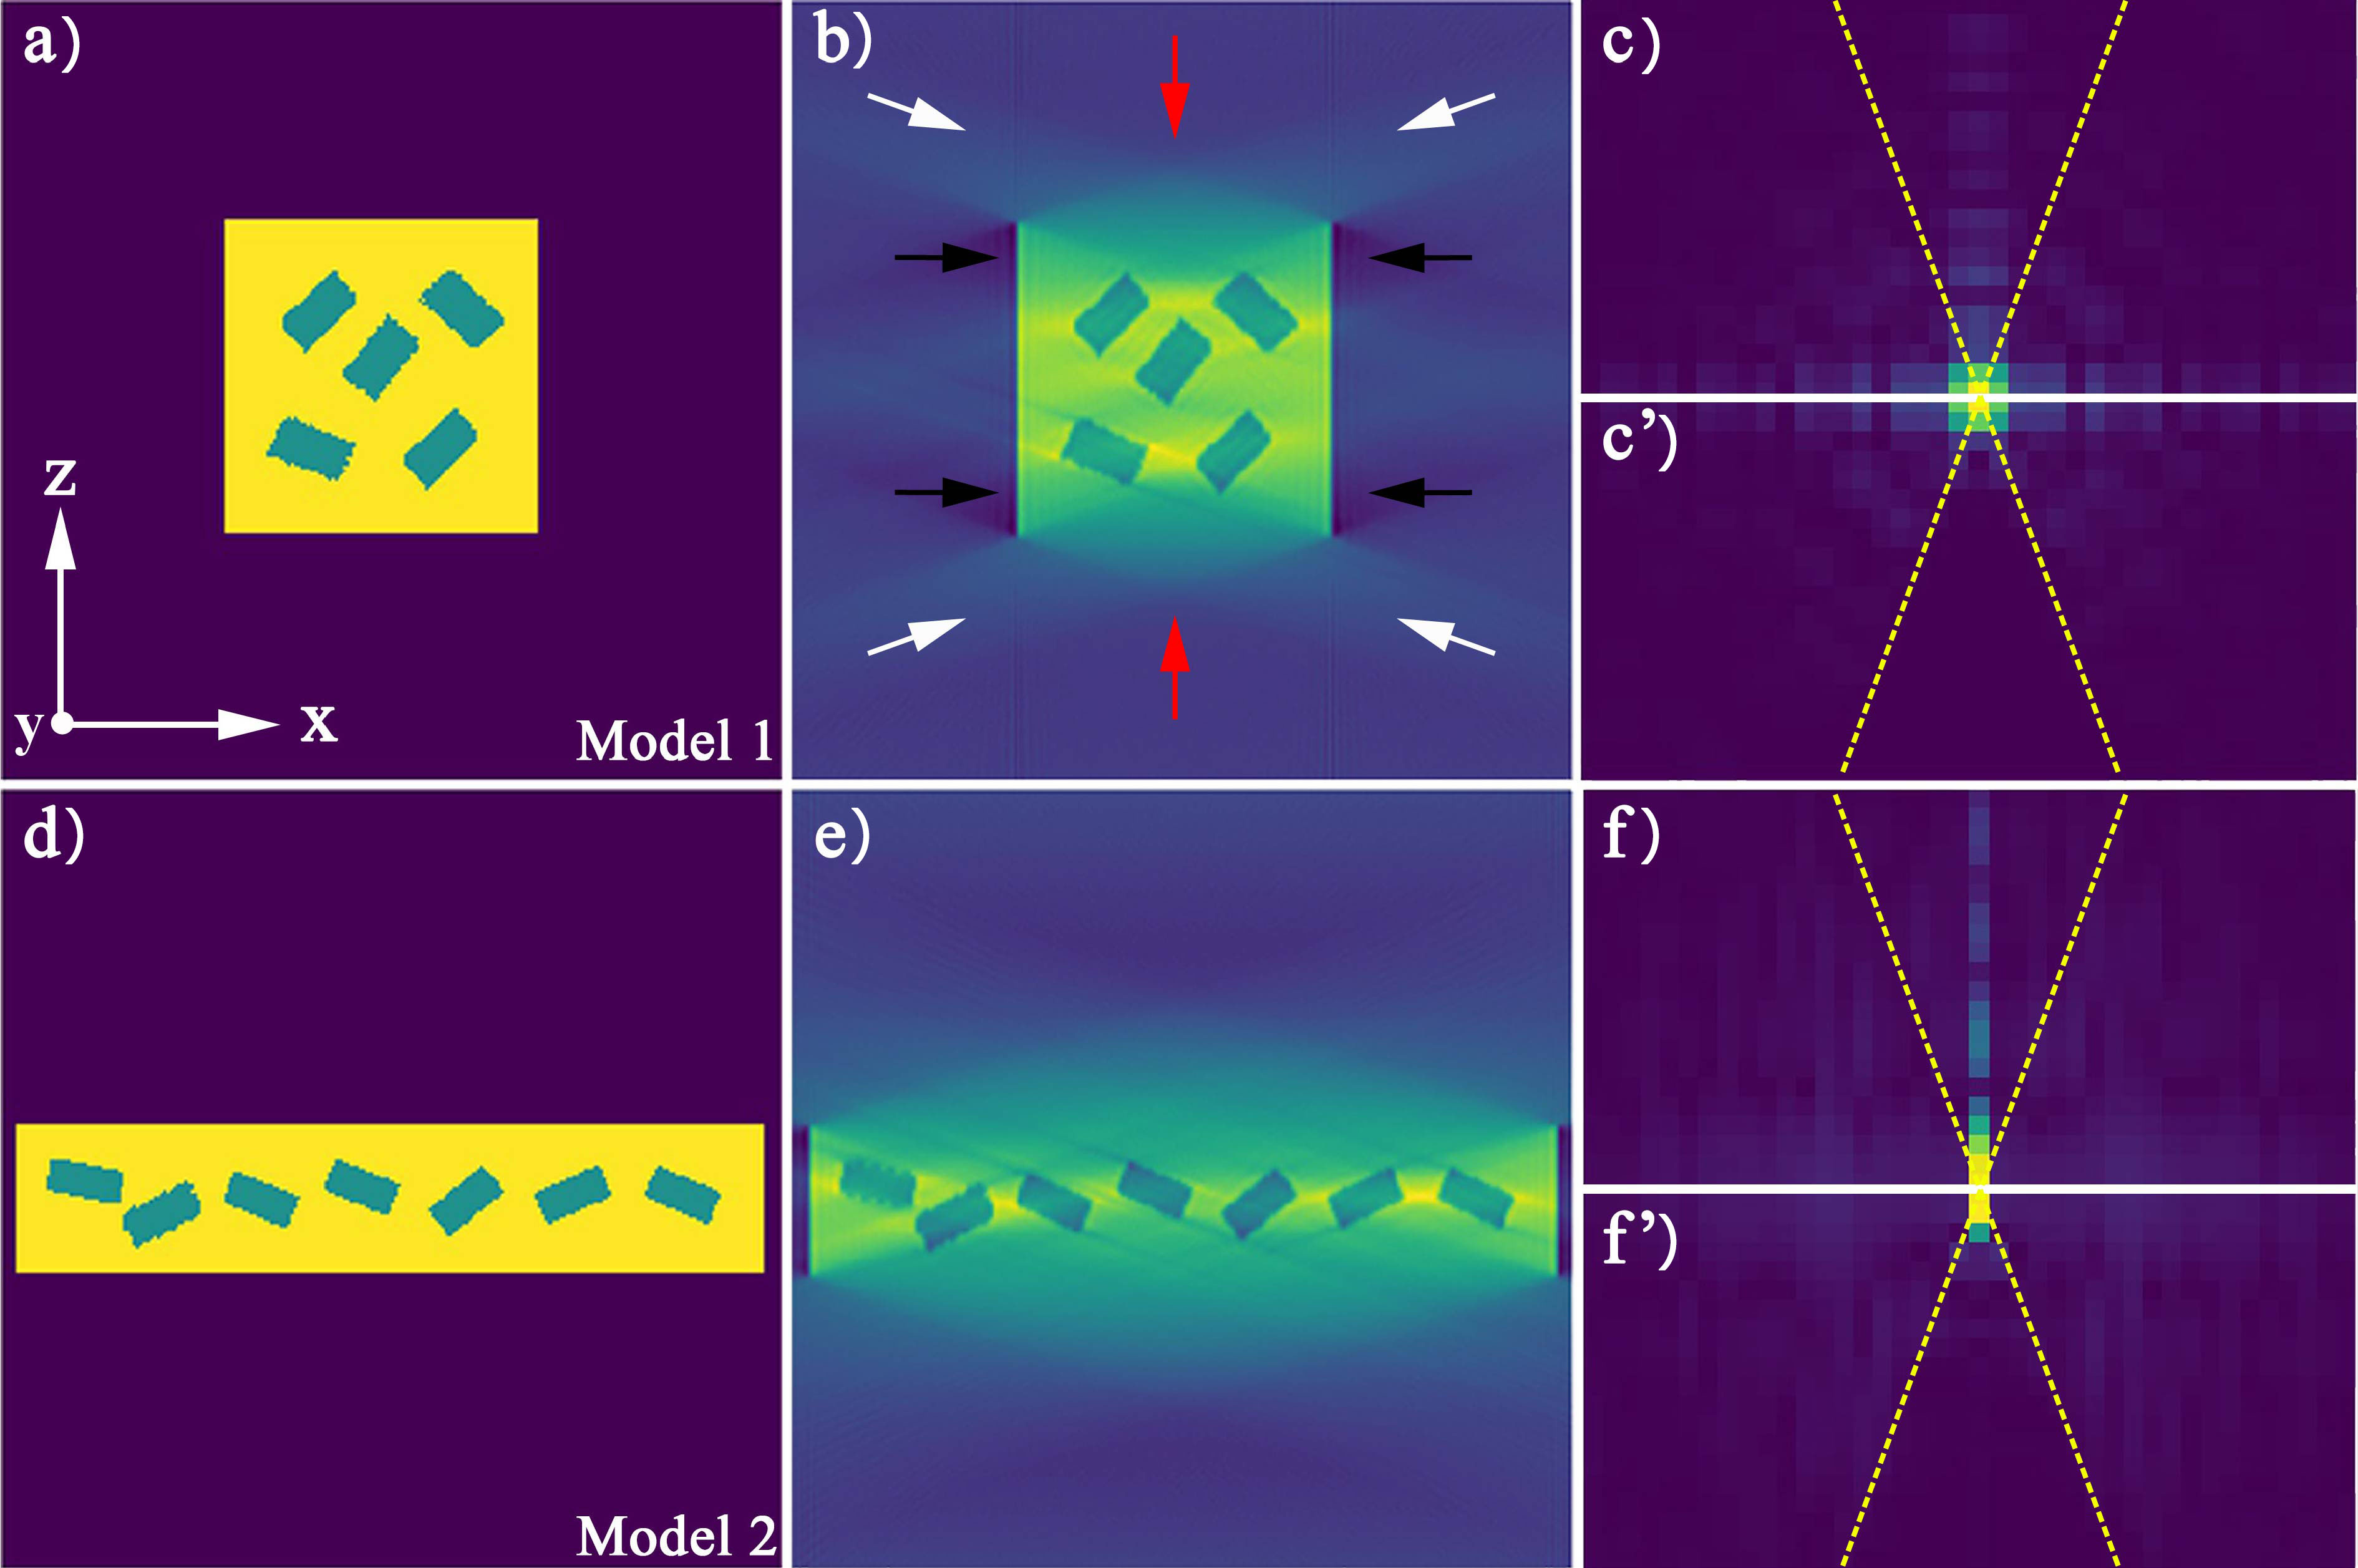
\includegraphics[width=0.9\textwidth]{../3.1/31}
	\caption{TEM 中严重的缺失锥假象图解}\label{fig:31}
	\song\tuzhu{a,d) 模型 1 和模型 2;b,e) 模型 1 和模型 2 的 sinograms 经 SIRT 重构的结果,迭代次数是 100 次,倾转角范围是 -70° 到 +70°,倾转间隔为 1°;c,f) 图 a 和 b 的傅里叶变换(仅显示中心上半部分);c',f') 图 b 和 e 的傅里叶变换(仅显示中心下半部分)}
\end{figure}

\section{NNART 算法和算法测试}
\subsection{算法介绍}

本章提出的 NNART 算法基于广泛使用的反传播神经网络模型~\cite{Rumelhart1986}求解线性方程组:$\boldsymbol{A}\boldsymbol{x}=\boldsymbol{b}$(详情见公式 1.43)。一般,ART 算法的重构过程是使用误差矫正,在迭代过程中使初始值(零或者猜测值)慢慢逼近线性方程组的解。在此基础上,NNART 借助神经网络来完成误差矫正过程,图 2.2a 是 NNART 的流程图。重构的每一次迭代分成三个部分:(i)一个五层的前馈神经网络,如图 2.2b 所示,它的输出层 $\boldsymbol{L}^{(4)}$ 是对应于公式(1.43)中 $\boldsymbol{x}$ 的一维的预测结果;(ii)通过坐标变换得到二维的预测结果,并将其投影,获得 sinogram;(iii)计算损失(loss),然后通过自适应梯度下降算法(adaptive  gradient descent,AdaGrad)优化神经网络中的权重和偏置,使下次迭代中的预测结果更接近正确解。在该算法中,实验投影 sinogram 数据,$\boldsymbol{S}^{exp}$,是在重构时唯一需要获知的信息。重构开始时,算法将使用随机变量对神经网络(包括输入层)进行初始化,当迭代达到一定次数 $t_{max}$ 时重构结束(结束时要保证 loss 收敛)。不过,一次重构的结果往往具有非常大的噪音(如图 2.16a 和 g),这是数值算法本身导致的噪音。为了获得平化解,本算法采用了多次重构取平均值的方法来获得最终结果 $\boldsymbol{I}_{avg}$,其中每次重构的初始化变量都取不同的随机数值。在本章第 2.3 和 2.4 节的研究中,全都取重构 20 次的平均结果。本算法并没有采用更为常用的正则化方法求平滑解~\cite{Aganj2007,Cichocki1995,Skoglund1996},因为探究发现 NNART 在结合了正则化项后,应用时总是受限,这会在第 2.5 节中说明。

\begin{figure}[htbp]
	\vspace{\baselineskip}
	\centering
	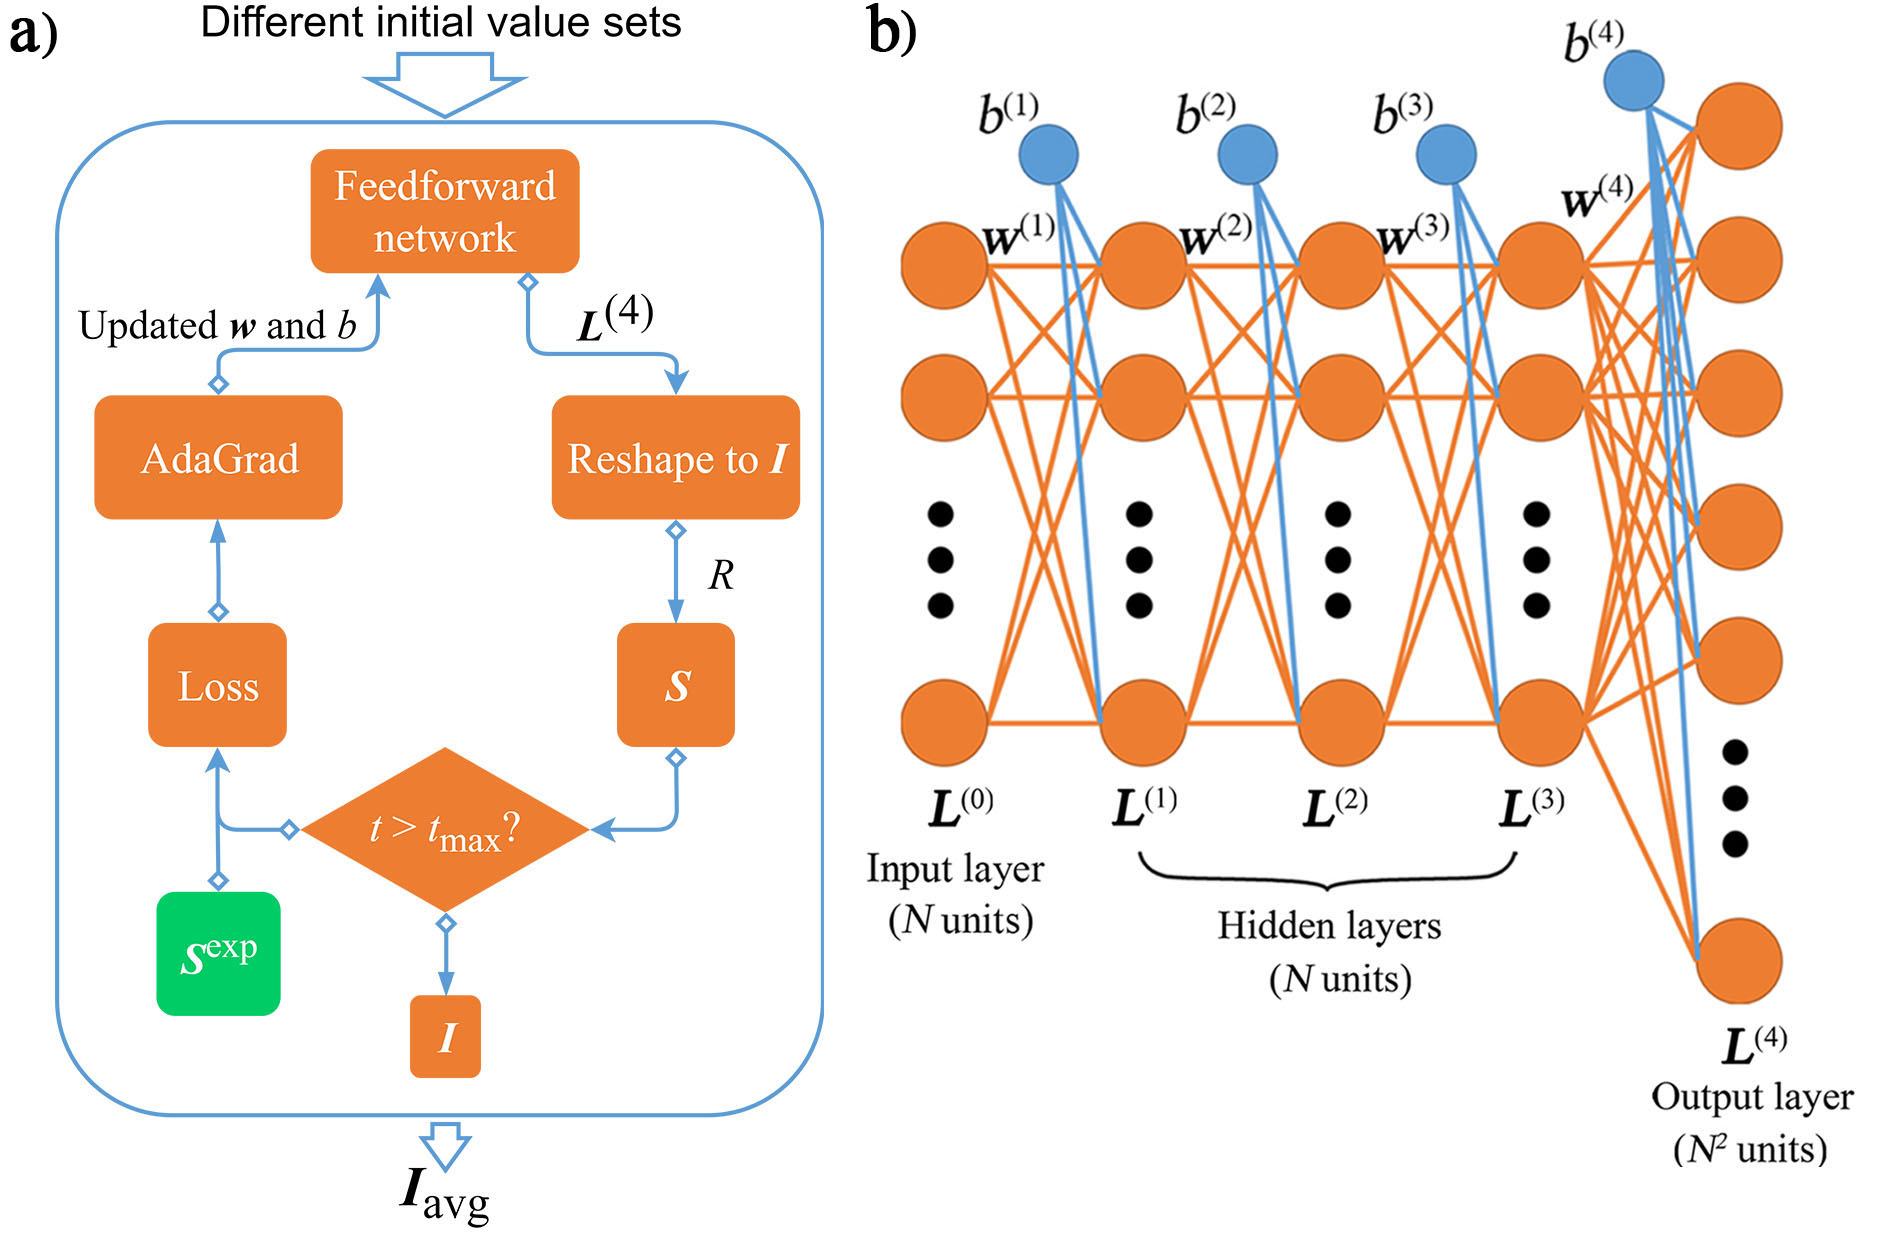
\includegraphics[width=0.9\textwidth]{../3.2/32}
	\caption{NNART 算法示意图}\label{fig:32}
	\song\tuzhu{a) NNART 算法流程图;b) 全连接前馈神经网络的示意图}
\end{figure}

图 2.2b 展示了 NNART 中使用的五层全连接前馈神经网络示意图,它的维度是 $N-N-N-N-N^2$,其中 $N\times N$ 是所需重构的图像的维度。输入层 $\boldsymbol{L}^{(0)}$ 以及所有的权重和偏置将根据截断正态分布的概率进行初始化。相邻两层之间的前向传播公式如下:
\begin{equation}
	\boldsymbol{L}^{(n)}= \sigma \left(\boldsymbol{L}^{(n-1)}\times \boldsymbol{w}^{(n)} + b^{(n)}\right)
\end{equation}
其中 $\boldsymbol{w}^{(n)}$ 和 $b^{(n)}$ 是连接相邻两层的权重和偏置,$\sigma$ 是非线性激活函数,本算法中使用的是 Relu 函数:
\begin{equation}
\sigma(x)= \max(x,0)
\end{equation}
为了实现神经网络的全连接,$\boldsymbol{w}^{(n)}(n = 1, 2, 3)$ 的维度是 $N\times N$ 而 $\boldsymbol{w}^{(4)}$ 的维度是 $N\times N^2$。$b^{(n)} (n = 1\sim 4)$ 是标量变量。

然后,输出层 $\boldsymbol{L}^{(4)}$ 中的元素的坐标会被重新排列得到预测的重构结果 $\boldsymbol{I}$:
\begin{equation}
	\boldsymbol{I}_{[k/N],mod(k,N)}=\boldsymbol{L}^{(4)}_k,k\in Z,0\le k<N^2
\end{equation}
接着,图像 $\boldsymbol{I}$ 通过拉登变换($\mathcal{R}$)进行投影得到 sinogram, $\boldsymbol{S}$:
\begin{equation}
 \boldsymbol{S}=\mathcal{R}(\boldsymbol{I})
\end{equation}
损失函数定义为实验投影 $\boldsymbol{S}^{exp}$ 与预测投影 $\boldsymbol{S}$ 之间的绝对误差的根号的求和:
\begin{equation}
L=\sum \sqrt{|\boldsymbol{S} - \boldsymbol{S}^{exp}|}
\end{equation}
最后,根据梯度下降法,沿着使损失 $L$ 变小的梯度更新权重和偏置,使下次迭代中的预测结果更接近正确解,梯度下降法的公式如下:
\begin{equation}
w^{(n)(t+1)}_{i,j}=w^{(n)(t)}_{i,j}-\eta \left.\frac{\partial L}{\partial w^{(n)}_{i,j}}\right|_{w^{(t)}}
\end{equation}
\begin{equation}
b^{(n)(t+1)}=b^{(n)(t)}-\eta \left.\frac{\partial L}{\partial b^{(n)}}\right|_{b^{(t)}}
\end{equation}
其中 $t$ 是迭代次数,$\eta$ 是学习率。在本算法中,使用了自适应梯度下降算法,它在迭代过程中能够自动调整学习率。

本章中 NNART 的实现使用了自研的 Python 代码,其中神经网络的运算通过 Tensorflow~\cite{Abadi2016} 模块实现。

\subsection{重构过程}
本条以模型 1 为例,详细描述 NNART 的重构过程,促进对其重构原理的理解。原始模型如图 2.1a 所示,像素大小是 $256\times 256$,然后模型在 -70° 至 +70° 的倾转角,倾转间隔为 1° 的条件下被投影。随后,投影数据使用 NNART 进行重构,重构结果如图 2.3 所示。

图 2.3a 展示了重构过程中 loss 的收敛曲线(纵坐标使用对数标尺)。由于重构开始时的神经网络是随机赋值初始化的,所以预测结果和真实的实验数据之间的偏差非常大,loss 值接近 10$^4$。随后,loss 在若干次迭代内大幅度下降,这意味着该过程中权重和偏置的变化幅度很大。尽管如此,如图 2.3b 所示,此时的预测结果仍然呈现随机噪音。当迭代次数到达 40 次后,loss 下降的速度将减缓。此时的重构结果,正方形样品的大致轮廓开始出现,且相较于图 2.3b 噪音减少了很多,但是样品的内部细节还没有展现出来。图 2.3d 展示了迭代次数到达 400 次时的重构结果。在这个阶段,重构结果和模型 1(图2.1a)接近了很多,但是此时存在着相当严重的射线和伸长假象,而且重构对象的边界非常模糊。不过,暗影假象已经得到了一定程度的抑制,而且图像的背景非常干净,几乎没有噪音。最后,在迭代次数到达 3000 次时,loss 收敛,重构结束。图 2.3e 展示了最终的重构结果,重构对象的边界和和内部的截面都非常清晰,而且缺失锥假象几乎被去除了。

\begin{figure}[htbp]
	\vspace{\baselineskip}
	\centering
	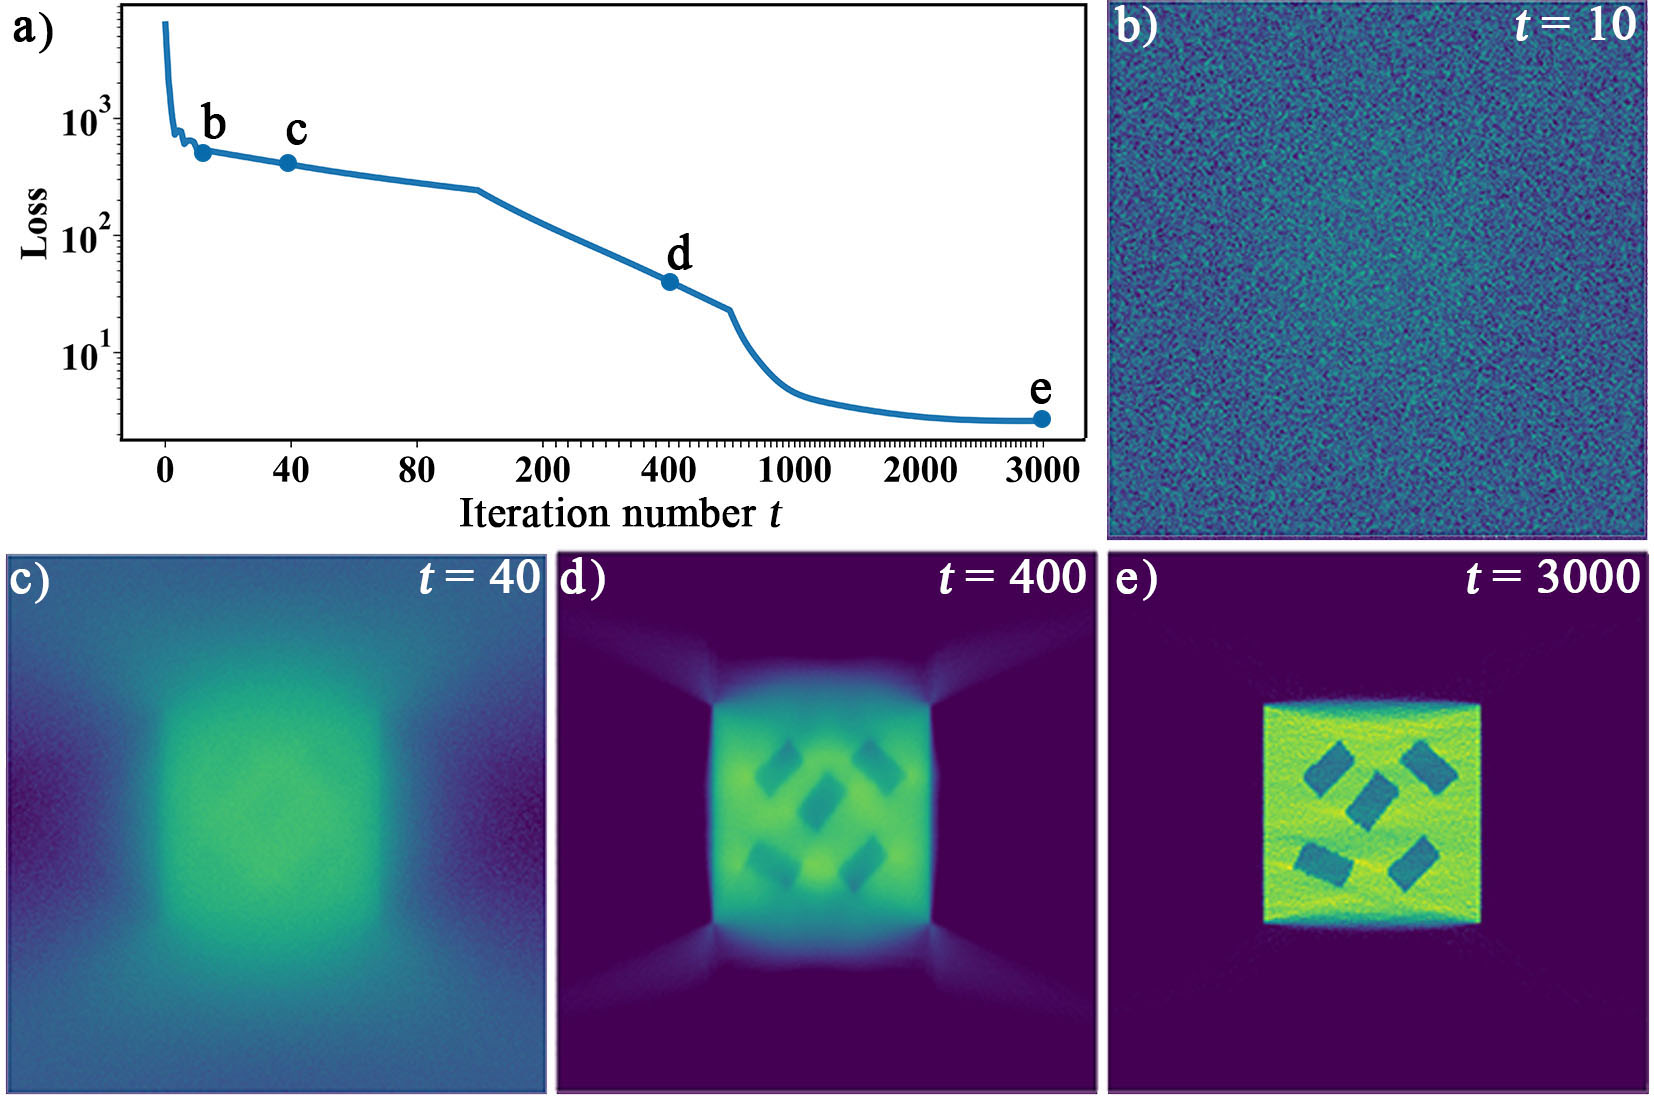
\includegraphics[width=0.9\textwidth]{../3.3/33}
	\caption{NNART 的重构过程}\label{fig:33}
	\song\tuzhu{a) 重构过程中 loss 的收敛曲线,其中纵轴是对数坐标;b-e) 不同迭代次数的重构结果:b) 10,c) 40,d) 400,e) 3000;图 a-e 都是 20 次重构平均的结果}
\end{figure}

图 2.4a-e 对比了模型 1(图2.1a)和图 2.3b-e 中的重构结果的傅里叶变换(仅展示中心右半部分)。显然,随着迭代次数的增加,重构的信息逐渐增多,并且缺失锥中的信息也在一定程度上被重构出来。图 2.4f 定量地对比了图 2.4a-e 沿 $z$ 方向的重构信息的强度。在迭代次数到达 400 时,如图 2.4d 所示,缺失锥以外的区域已经在一定程度上恢复出一些信息,但是沿 $z$ 方向重构的信息仍极为有限的。最终 3000 次迭代恢复出的信息和模型 1 沿 $z$ 方向的信息在低频部分相当接近,并且在高频部分仍具有和模型 1 相同的趋势,这说明重构的信息是正确的。但是,重构的信息沿着 $z$ 方向最终会衰减至无,所以 NNART 无法重构出更高频率的信息,所以在 $z$ 方向上的重构分辨率依然将低于 $x$ 方向的重构分辨率。

总体而言,NNART 在抑制缺失锥假象上的效果是非常显著的,它能够正确地恢复出缺失锥中的信息。这种优异的性能应归功于复杂的神经网络。因为在 NNART 的每一次迭代中,实验数据的信息将通过神经网络的非线性变换,被映射到高维空间中(~$\sim N^3$ 维度的神经网络),然后再经梯度下降算法和前馈传播,对重构结果进行修正。这种先升维再降维的方式,相比于仅在低维空间进行误差修正的 ART 算法,具有更好的求解效果,所以即使没有使用任何先验知识,也能抑制缺失锥假象。

\begin{figure}[htbp]
	\vspace{\baselineskip}
	\centering
	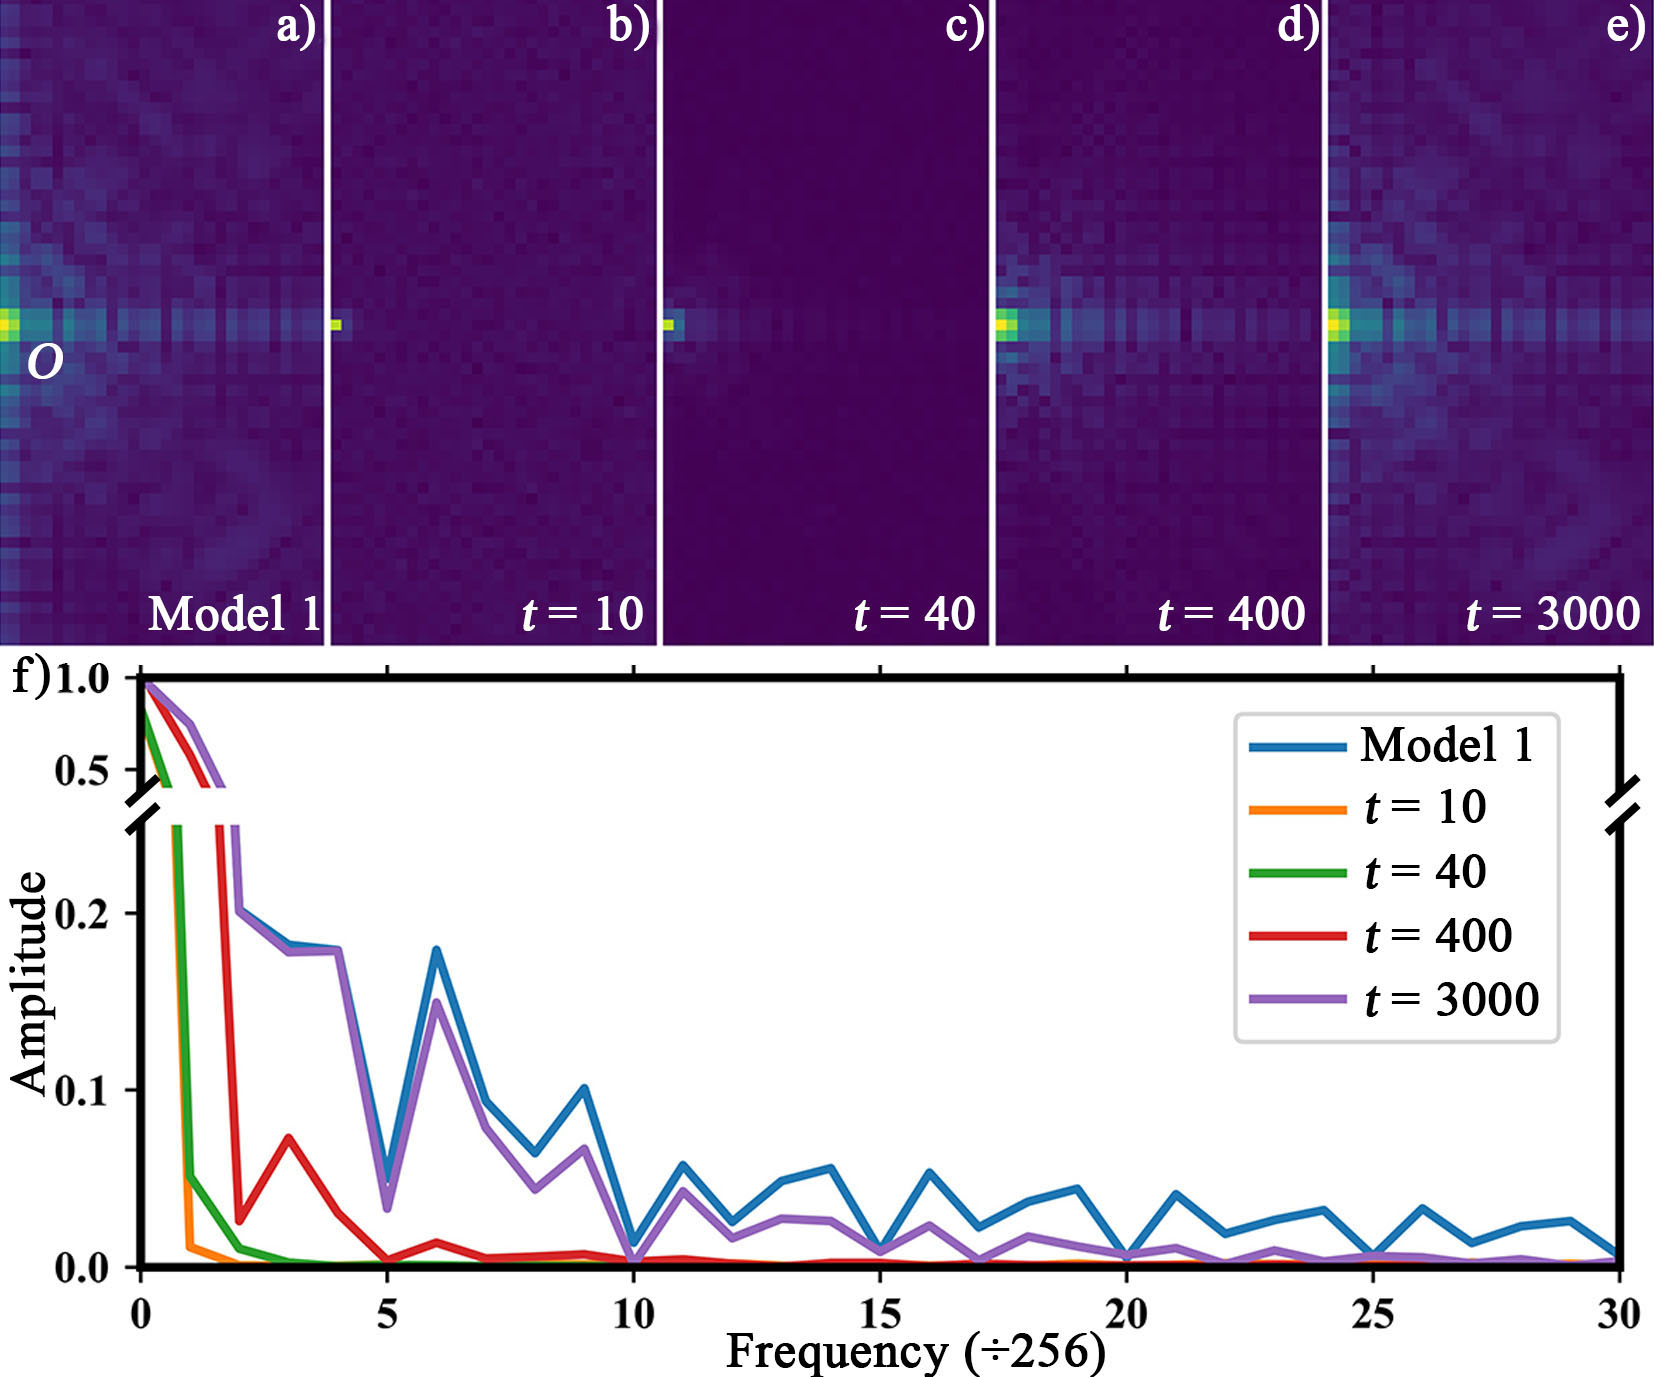
\includegraphics[width=0.9\textwidth]{../3.4/34}
	\caption{不同迭代次数的重构结果的傅里叶变换及分析}\label{fig:34}
	\song\tuzhu{a) 模型 1 的傅里叶变换;b-e) 迭代次数分别维 10,40,400,3000 的重构结果的傅里叶变换;傅里叶变换仅展示了中心右半部分(60  像素 $\times $ 30 像素),且显示于同一灰度衬度下;f) 图 a-e 沿 $z$ 轴的振幅对比曲线}
\end{figure}

\subsection{模拟测试}
图 2.5 展示了不同倾转角范围下,用两种算法重构模型 2 的结果。图 2.5a 和 e 说明了当倾转角范围是 -70° 至 70° 时,NNART 和 TVM 均能有效抑制缺失锥假象。当倾转角范围减小时,图 2.5b-d 和 f-h 中的重构结果中沿 $z$ 方向的伸长假象都会变严重,而且内部的矩形会丢失一些局部细节,不过整个模型都能保持完整。而且,内部的小矩形产生的射线假象变得越来越严重,在 TVM 的重构结果中,这些假象会使结果的补丁状样貌更加明显。相对而言,TVM 抑制伸长假象的效果不及 NNART,而且图 2.5f-h 中在拉伸假象的边界上还存在明显的暗衬度。相反,NNART 的重构结果的总体形状与模型 2 更加接近,而且整体观感比 TVM 的结果更清晰。不过,在 NNART 的重构结果中,当倾转角范围变小后,某些内部小矩形的角上出现了一些小孔,如图 2.5b-d 中白色箭头所标注。这些孔洞的出现,是神经网络的过拟合造成的。当实验数据减少时,过拟合更容易发生,此时神经网络可能会把一些细节当作特征放大。

\begin{figure}[htbp]
	\vspace{\baselineskip}
	\centering
	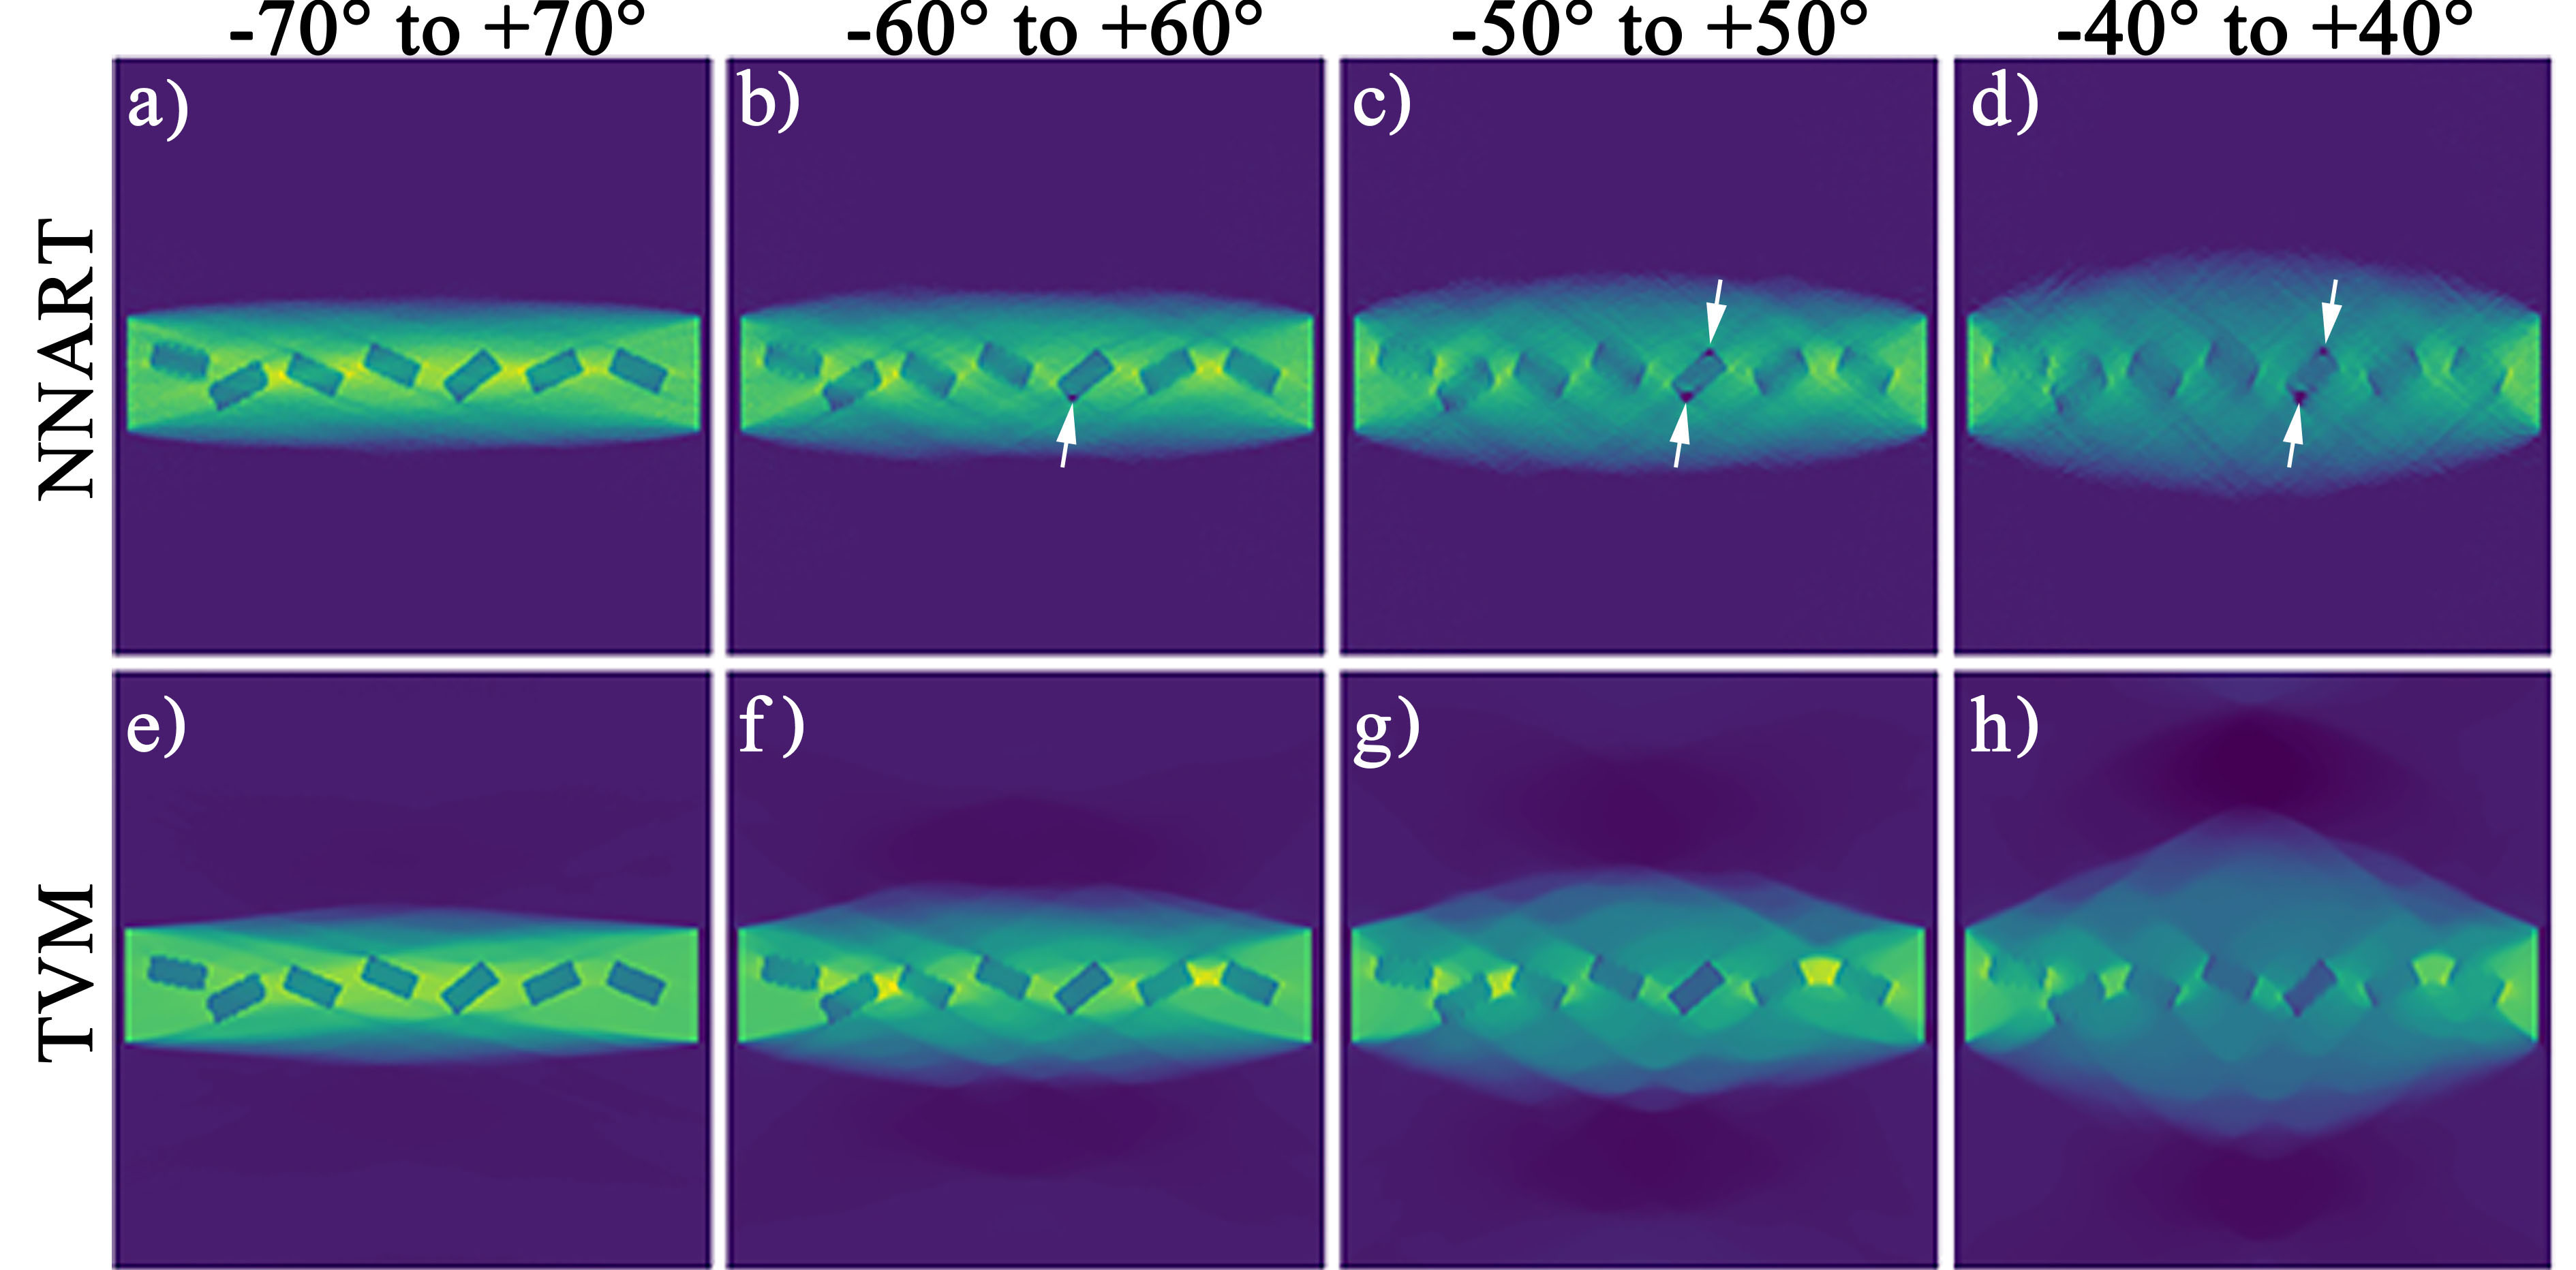
\includegraphics[width=0.9\textwidth]{../3.5/35}
	\caption{不同倾转角范围下 NNART 和 TVM 重构结果对比}\label{fig:35}
	\song\tuzhu{其中倾转角范围分别是:a,e) -70° 至 +70°;b,f) -60° 至 +60°;c,g) -50° 至 +50°;d,h) -40° 至 +40°;倾转间隔均为 1°,NNART 和 TVM 的迭代次数分别是 6000 次和 5000 次,以保证算法收敛;所有图像均显示于同一灰度衬度进行对比}
\end{figure}

噪音是一个无法在实验中避免的降低重构质量的因素。特别地,噪音是否会影响算法对缺失锥假象的抑制,是一个需要在此重点考虑的问题。图 2.6a 和 d 展示了在模型 2 的 sinogram 中加入信噪比(signal noise ratio,SNR)分别为 30 和 20 的泊松噪音后的局部图像。图 2.6b,e,c,f 展示了使用 NNART 和 TVM 重构倾转角范围为 -60° 至 +60° 的带有噪音的 sinogram 的结果。很显然,相比于无噪音时的重构结果(图 2.5b 和 f),不同程度的噪音出现在了相应的重构结果中。不过,对于 NNART 的重构结果而言,图 2.6b 和 e 与图 2.5b 相比,除了噪音没有明显的不同,这意味着噪音并不影响 NNART 对缺失锥假象的抑制作用。反观 TVM 的重构结果,当信噪比是 20 时,整个重构图像中都有严重的噪音,连原有的补丁状特征都消失了,而且块体模型也变得难以辨认。

以上结果证明 NNART 据有非常好的抗噪音能力,其原因可分为两点:首先,
如第 2.2.2 条中所述,复杂的神经网络使得重构更有效。其次,NNART 中使用多次重构平均的方法来求解平滑解,而非使用正则化等方法。使用多次重构平均的方法其实是通过统计的方式来去除数值算法带来的噪音。而因为实验数据是唯一的,所以多次重构平均方法和实验数据中本身存在的噪音是无关的,即实验数据中的噪音不容易影响到重构的过程。反观一些正则化方法无法避免正则化项对实验噪音的作用,所以实验噪音也会相应地影响重构结果。

\begin{figure}[H]
	\vspace{\baselineskip}
	\centering
	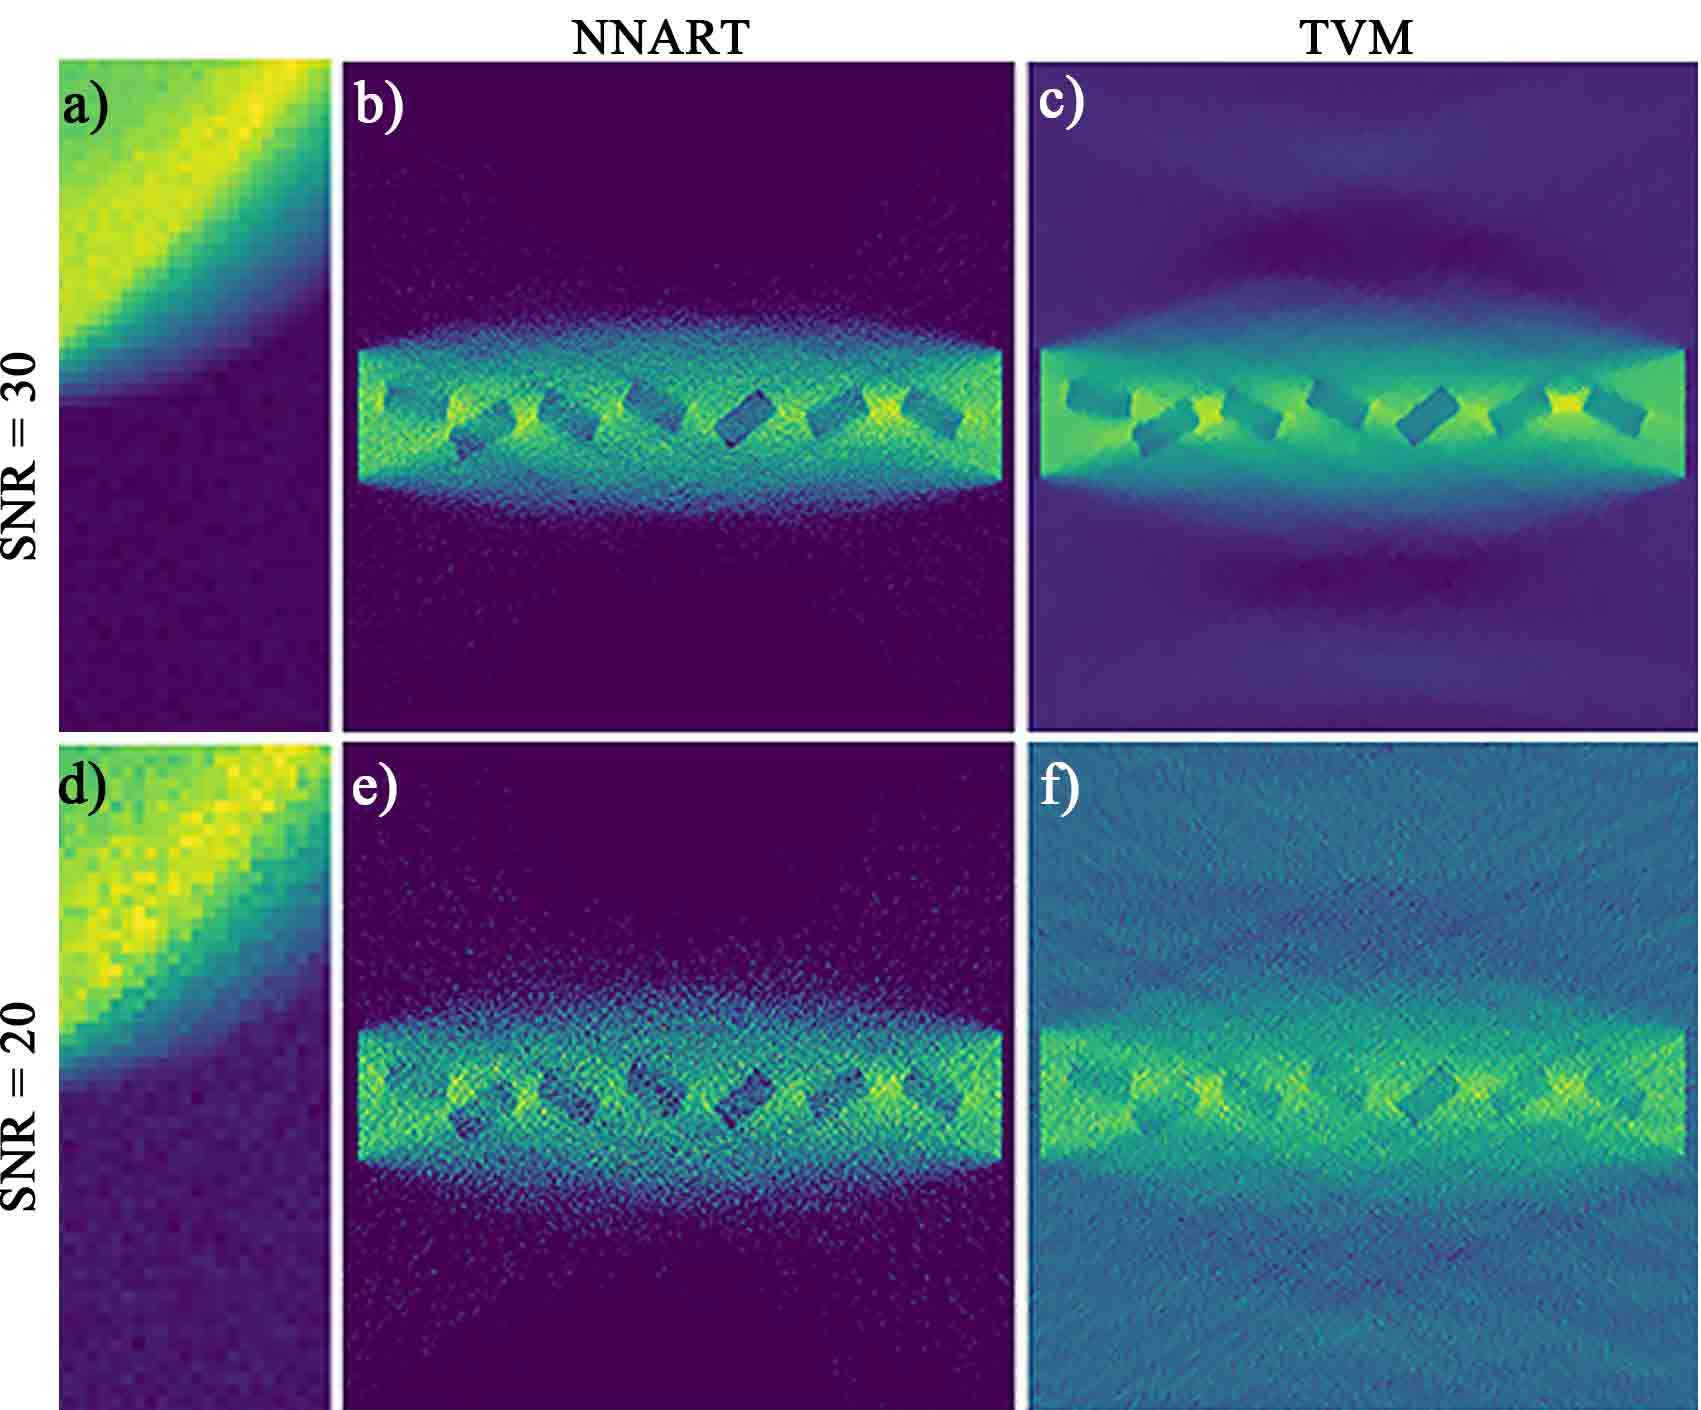
\includegraphics[width=0.9\textwidth]{../3.6/361}
	\caption{噪音对重构的影响}\label{fig:36}
	\song\tuzhu{a,d) 加入信噪比为 30 和 20 的泊松噪音后的 sinogram 的局部示意图;b,c) NNART 和 TVM 重构的加入信噪比为 30 的泊松噪音后的模型 2 的 sinogram 的结果;e,f) NNART 和 TVM 重构的加入信噪比为 20 的泊松噪音后的模型 2 的 sinogram 的结果;sinogram 的倾转角范围是 -60° 至 +60°}
\end{figure}

纳米颗粒是热门的研究对象。当许多纳米颗粒分散在某一区域中时,面对这些颗粒的投影强度的相互影响,NNART 是否还能正常地重构它们,并抑制缺失锥假象,也是一个值得探讨的问题。图 2.7c 是一簇纳米颗粒模型,颗粒形状是纵横比各异的圆角矩形,颗粒在图中呈不同强度,代表它们具有不同的元素成分。图 2.7a 和 b 分别是用 NNART 和 FBP 重构倾转角为 -70° 到 +70° 的 sinogram 的结果。在 FBP 的重构结果中,缺失锥假象非常严重,每个颗粒的两侧都有暗影假象,且射线假象和拉伸假象也很明显。而在图 2.7a 中,缺失锥假象得到了很好的控制,颗粒轮廓分明。对比图 2.7d-f,可知 NNART 重构了大部分缺失锥中原本丢失的信息,且图 2.7d 和 2.7f 非常相似。为了进一步分析恢复的信息的准确性,图 2.7g 和 h 定量对比了图 2.7d 和 f 沿 $z$ 轴和 $x$ 轴的强度。图 2.7h 中两条曲线吻合得很H,H,这是因为沿 $x$ 方向不存在缺失锥, NNART 能够非常准确地重构该方向上的信息。而在图 2.7g 中,沿 $z$ 方向,NNART 重构的信息的强度与原始的强度也基本吻合,仅在频率较高时开始衰减。所以,NNART 能够很好地重构纳米颗粒。


\begin{figure}[H]
	\vspace{\baselineskip}
	\centering
	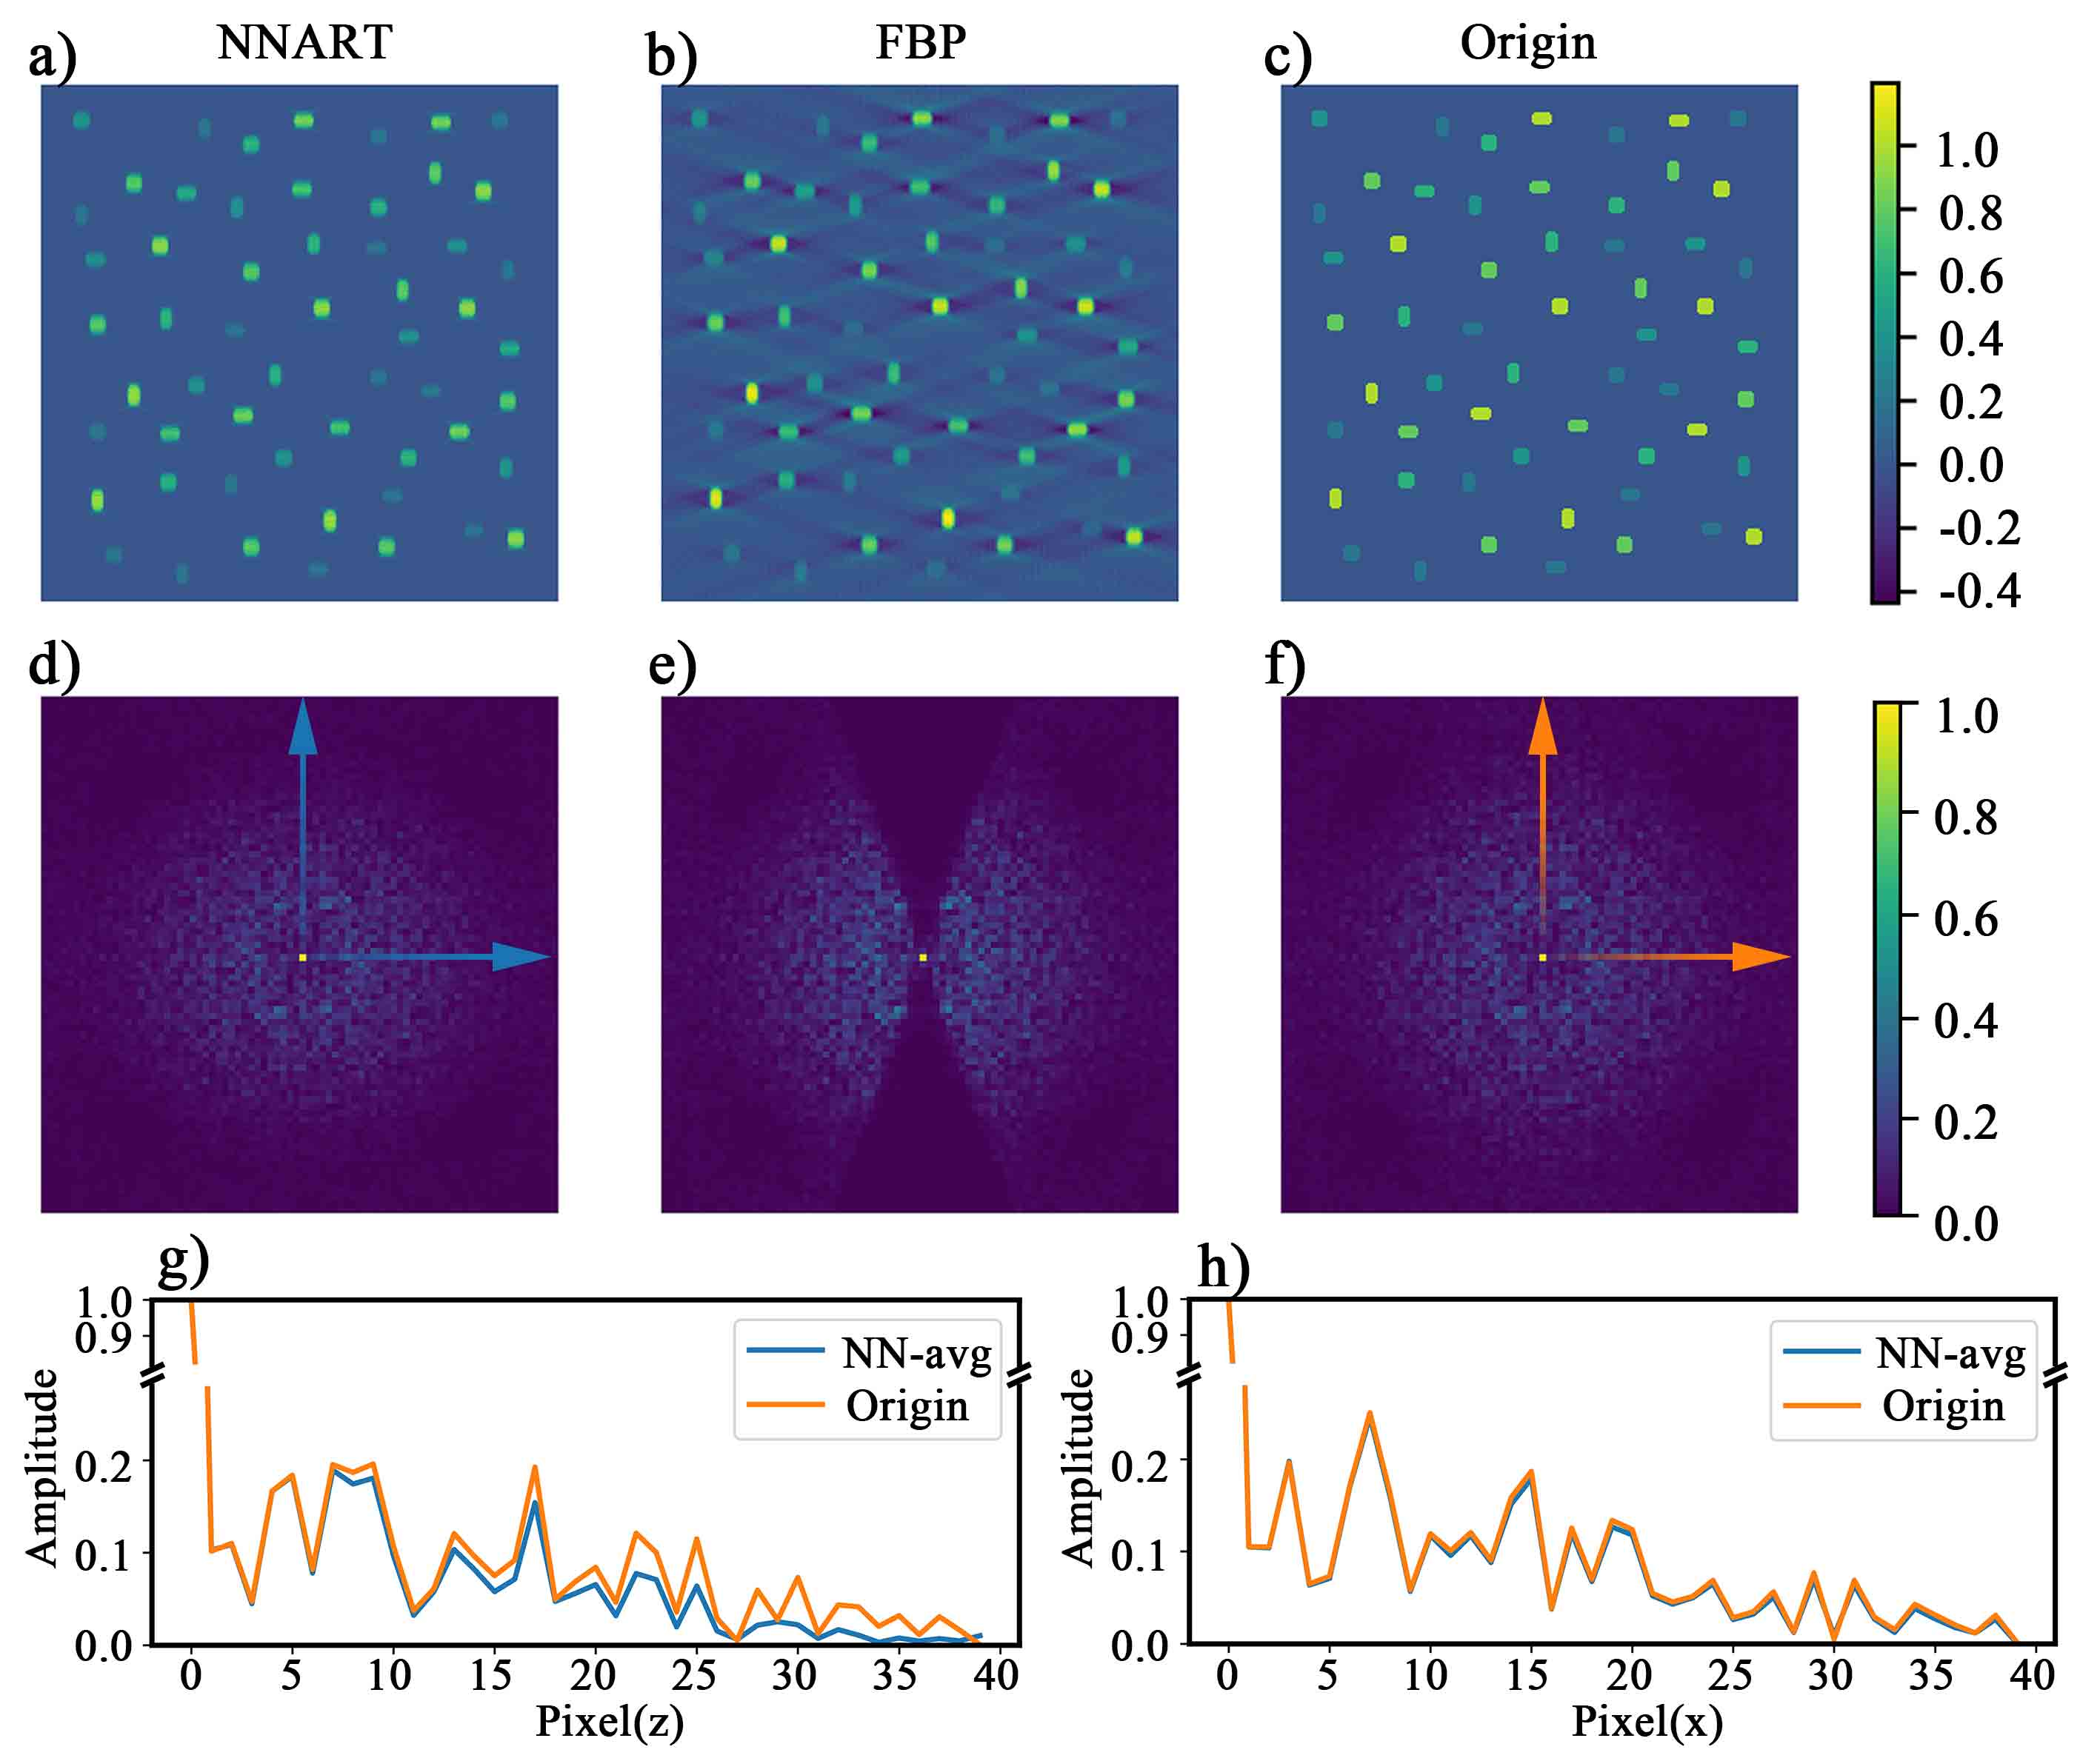
\includegraphics[width=0.9\textwidth]{../3.13/313}
	\caption{NNART 与 FBP 重构纳米颗粒模型的对比图}\label{fig:313}
	\song\tuzhu{a,b) NNART 和 FBP 重构纳米颗粒模型的结果;c) 纳米颗粒模型;d-f) a,b,c 的傅里叶变换;g,h) d 与 f图中沿 $z$ 轴和 $x$ 轴的强度对比图;重构的 sinogram 的倾转角范围是 -70° 到 +70°}
\end{figure}


本节还利用纳米颗粒模型,探究了极端情况下的重构情况。在 limited data 情形下,sinogram 的倾转角为 -70° 到 +70°,但间隔为 3°,投影数据缩减至原来的 1/3。此时,FBP 的重构结果(图 2.8b)中具有非常严重的条纹假象,在其傅里叶变换(图 2.8f)中也可明显地看出数据量的稀少(边缘出现条纹)。NNART 的重构结果的质量则高很多,没有出现条纹假象。而在 limited angle 情形下,sinogram 的倾转角为 -40° 到 +40°,间隔为 1°。此时 FBP 的重构结果中颗粒在 $z$ 方向上拉伸得特别明显,而 NNART 能够在一定程度上抑制这些假象,恢复出 $z$ 方向上的信息。从图 2.8i 的定量对比中可以看出,在两种情形下,缺失锥中的信息仍然被恢复出了一部分,尽管不如图 2.7g 中恢复的程度高。而在图 2.8j 中,可见在 limited data 情形下,即使在 $x$ 方向上,NNART 也无法完美恢复出频率信息,该结果符合预期。


\begin{figure}[H]
	\vspace{\baselineskip}
	\centering
	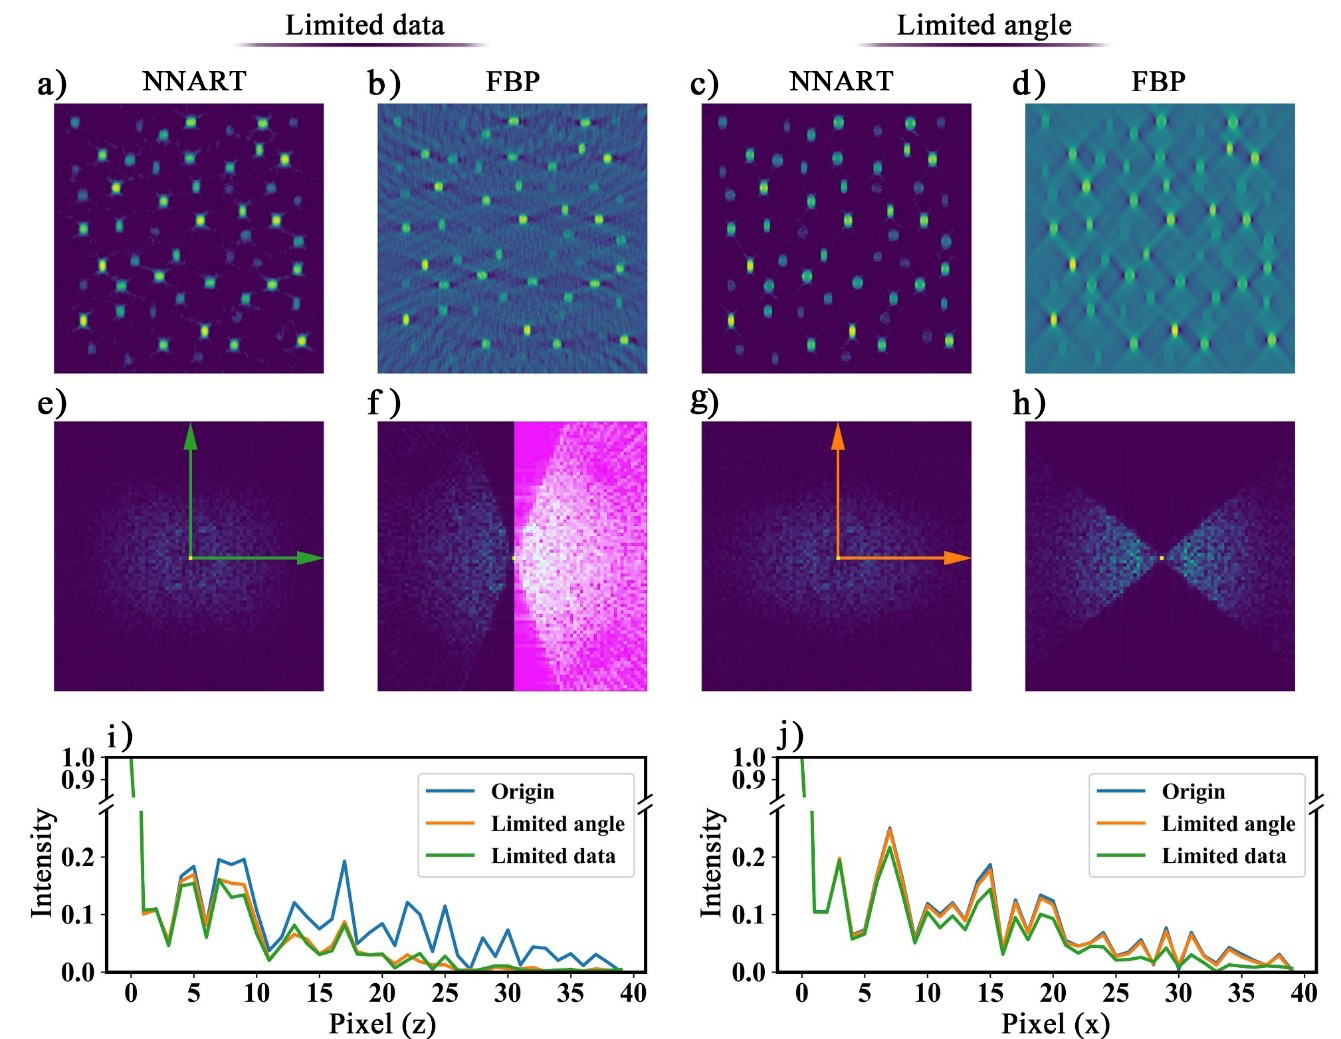
\includegraphics[width=0.9\textwidth]{../3.14/314}
	\caption{Limited data 和 limited angle 情形下纳米颗粒模型的重构结果对比}\label{fig:314}
	\song\tuzhu{a,b) Limited data 情形下 NNART 和 FBP 重构纳米颗粒模型的重构结果;c,d) Limited angle 情形下 NNART 和 FBP 重构纳米颗粒模型的重构结果;e-h) a,b,c,d 的傅里叶变换,f 右半边改变了图像衬度以更好地进行展示;i,j) e 和 g 与原始数据图 2.7f 中沿 $z$ 轴和 $x$ 轴的强度对比图;Limited data 情形下 sinogram 的倾转角为 -70° 到 70°,间隔为 3°;Limited angle 情形下的 sinogram 的倾转角为 -40° 到 40°,间隔为 1°}
\end{figure}

以上测试的模型中,强度都是分段不变的,下面以三个矩形模型为例,来探究当样品的成分分布具有梯度变化时 NNART 的重构效果。图 2.9d-f 是三个纵横比为 5 的矩形模型 rec1,rec2 和 rec3,其中 rec1 中的强度恒定,而 rec2 和 rec3 中的强度分别沿 $x$ 和 $z$ 轴呈梯度变化。在这种情况下,如图 2.9a-c 所示,在倾转角为 -70° 到 +70° 时,NNART 依然能够较好地重构矩形的整体形状,缺失锥假象被大幅抑制。不过,通过对比可见,图 2.9b 中矩形沿 $x$ 方向的强度变化在一定程度上被重构了出来,但是在图 2.9c 中则完全分辨不出强度是沿 $z$ 轴变化的。图 2.9g 和 h 是重构结果和原始模型的频率信息沿 $x$ 和 $z$ 轴的强度对比曲线。图 2.9g 证明 NNART 在重构 $x$ 方向的信息时是较为精确的。而在 2.9h 中,由于模型较大的纵横比,缺失锥范围内的信息在高频时较难被恢复,且当样品中的成分变化时,恢复的效果变差。正确重构物体的强度信息(成分)比重构物体的形状困难很多。特别地,当成分沿 $z$ 方向梯度变化时,这些频率信息将在缺失锥中丢失,更加难以复原。

\begin{figure}[H]
	\vspace{\baselineskip}
	\centering
	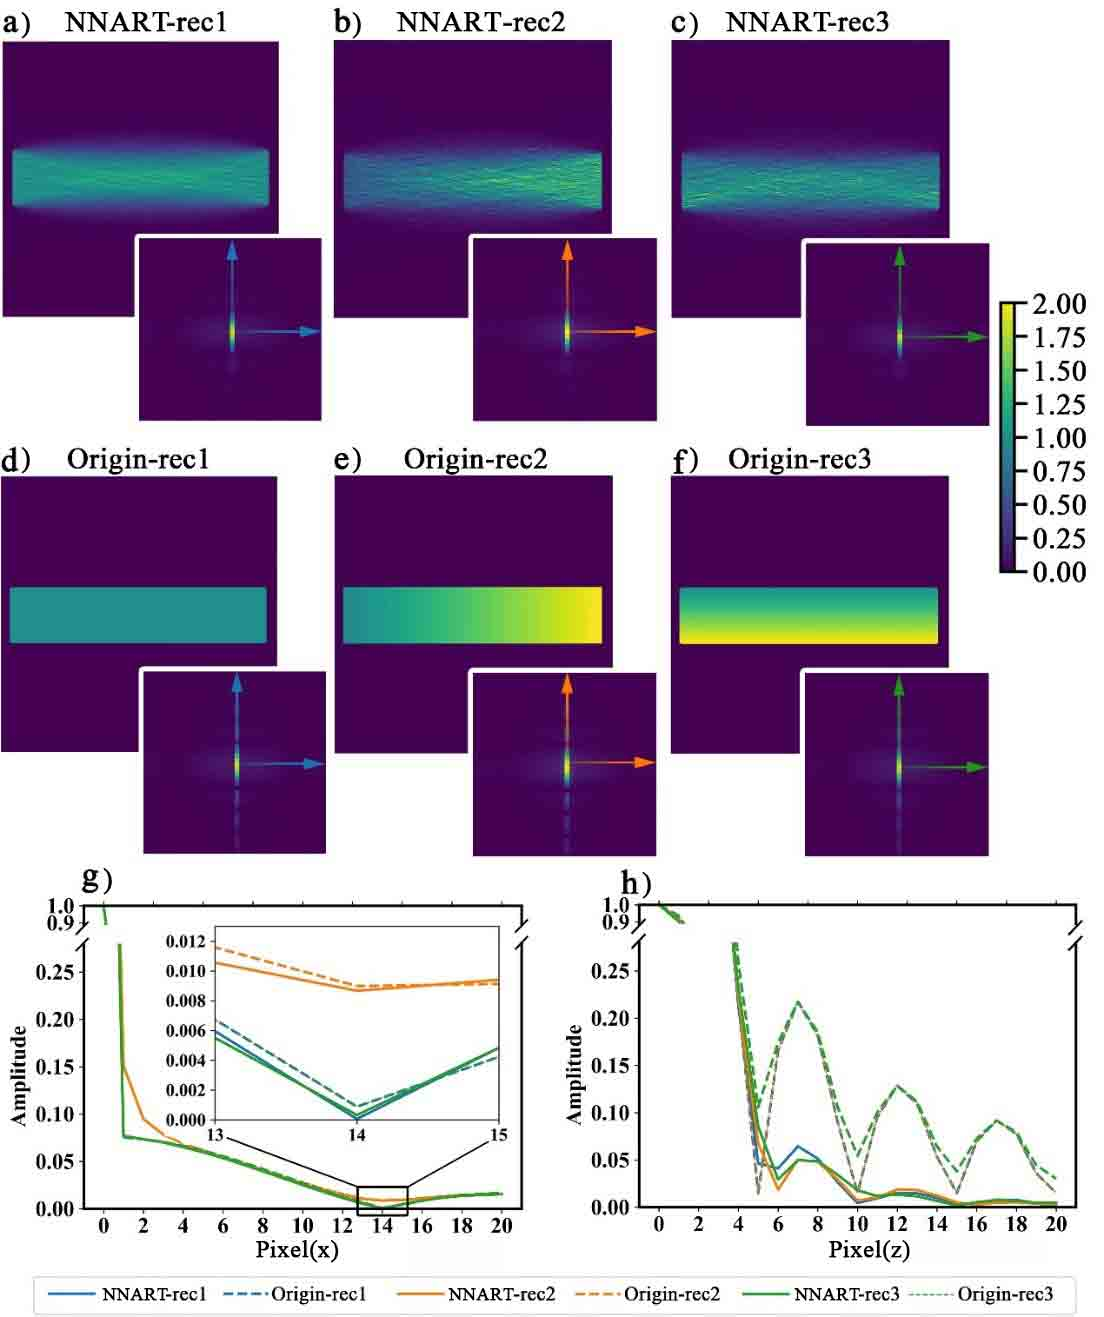
\includegraphics[width=0.9\textwidth]{../3.15/315}
	\caption{三个矩形模型与 NNART 的重构结果}\label{fig:314}
	\song\tuzhu{a-c) 纵横比为 5 的矩形模型 rec1,rec2 和 rec3 的 NNART 重构结果;d) 模型 rec1;e) 模型 rec2,强度沿 $x$ 方向梯度分布;f) 模型 rec3,强度沿 $z$ 方向梯度分布;g,h) 傅里叶空间中沿 $x$ 和 $z$ 轴的强度对比图;所有重构的倾转角范围是 -70° 到 +70°}
\end{figure}

另一个值得讨论的问题是,对于具有周期性的物体,其傅里叶空间的信息集中在固定的频率上。准确地恢复这些周期性的信息是检验 NNART 是否能抑制缺失锥假象和恢复缺失信息的一个很好的标准。图 2.10c 展示了一张模拟的 STEM 原子像,其中的原子在图像中周期性排列。它的傅里叶变换如图 2.10f 所示,其信息强度也是按周期性分布的。对该模型进行 -70° 至 +70° 的倾转投影得到带有缺失锥的 sinogram。图 2.10b 展示了使用 FBP 的重构结果,其中伸长假象和暗影假象非常明显。其傅里叶变换(图 2.10e)中 $z$ 轴上的信息完全缺失。而在 NNART 的重构结果(如图 2.10a 所示)中,原子的形状更接近圆形,暗影假象减弱很多。在它的傅里叶变换(图 2.10d)中,如红色箭头所示,缺失的信息被恢复。图 2.10g 和 h 定量对比了图 2.10d 和 f 沿 $x$ 和 $z$ 轴的强度,显然 NNART 完全恢复了沿 $x$ 轴的信息,而 $z$ 轴上的信息也在很大程度上被恢复出来,这说明 NNART 的确能够正确地恢复出缺失的信息。

\begin{figure}[H]
	\vspace{\baselineskip}
	\centering
	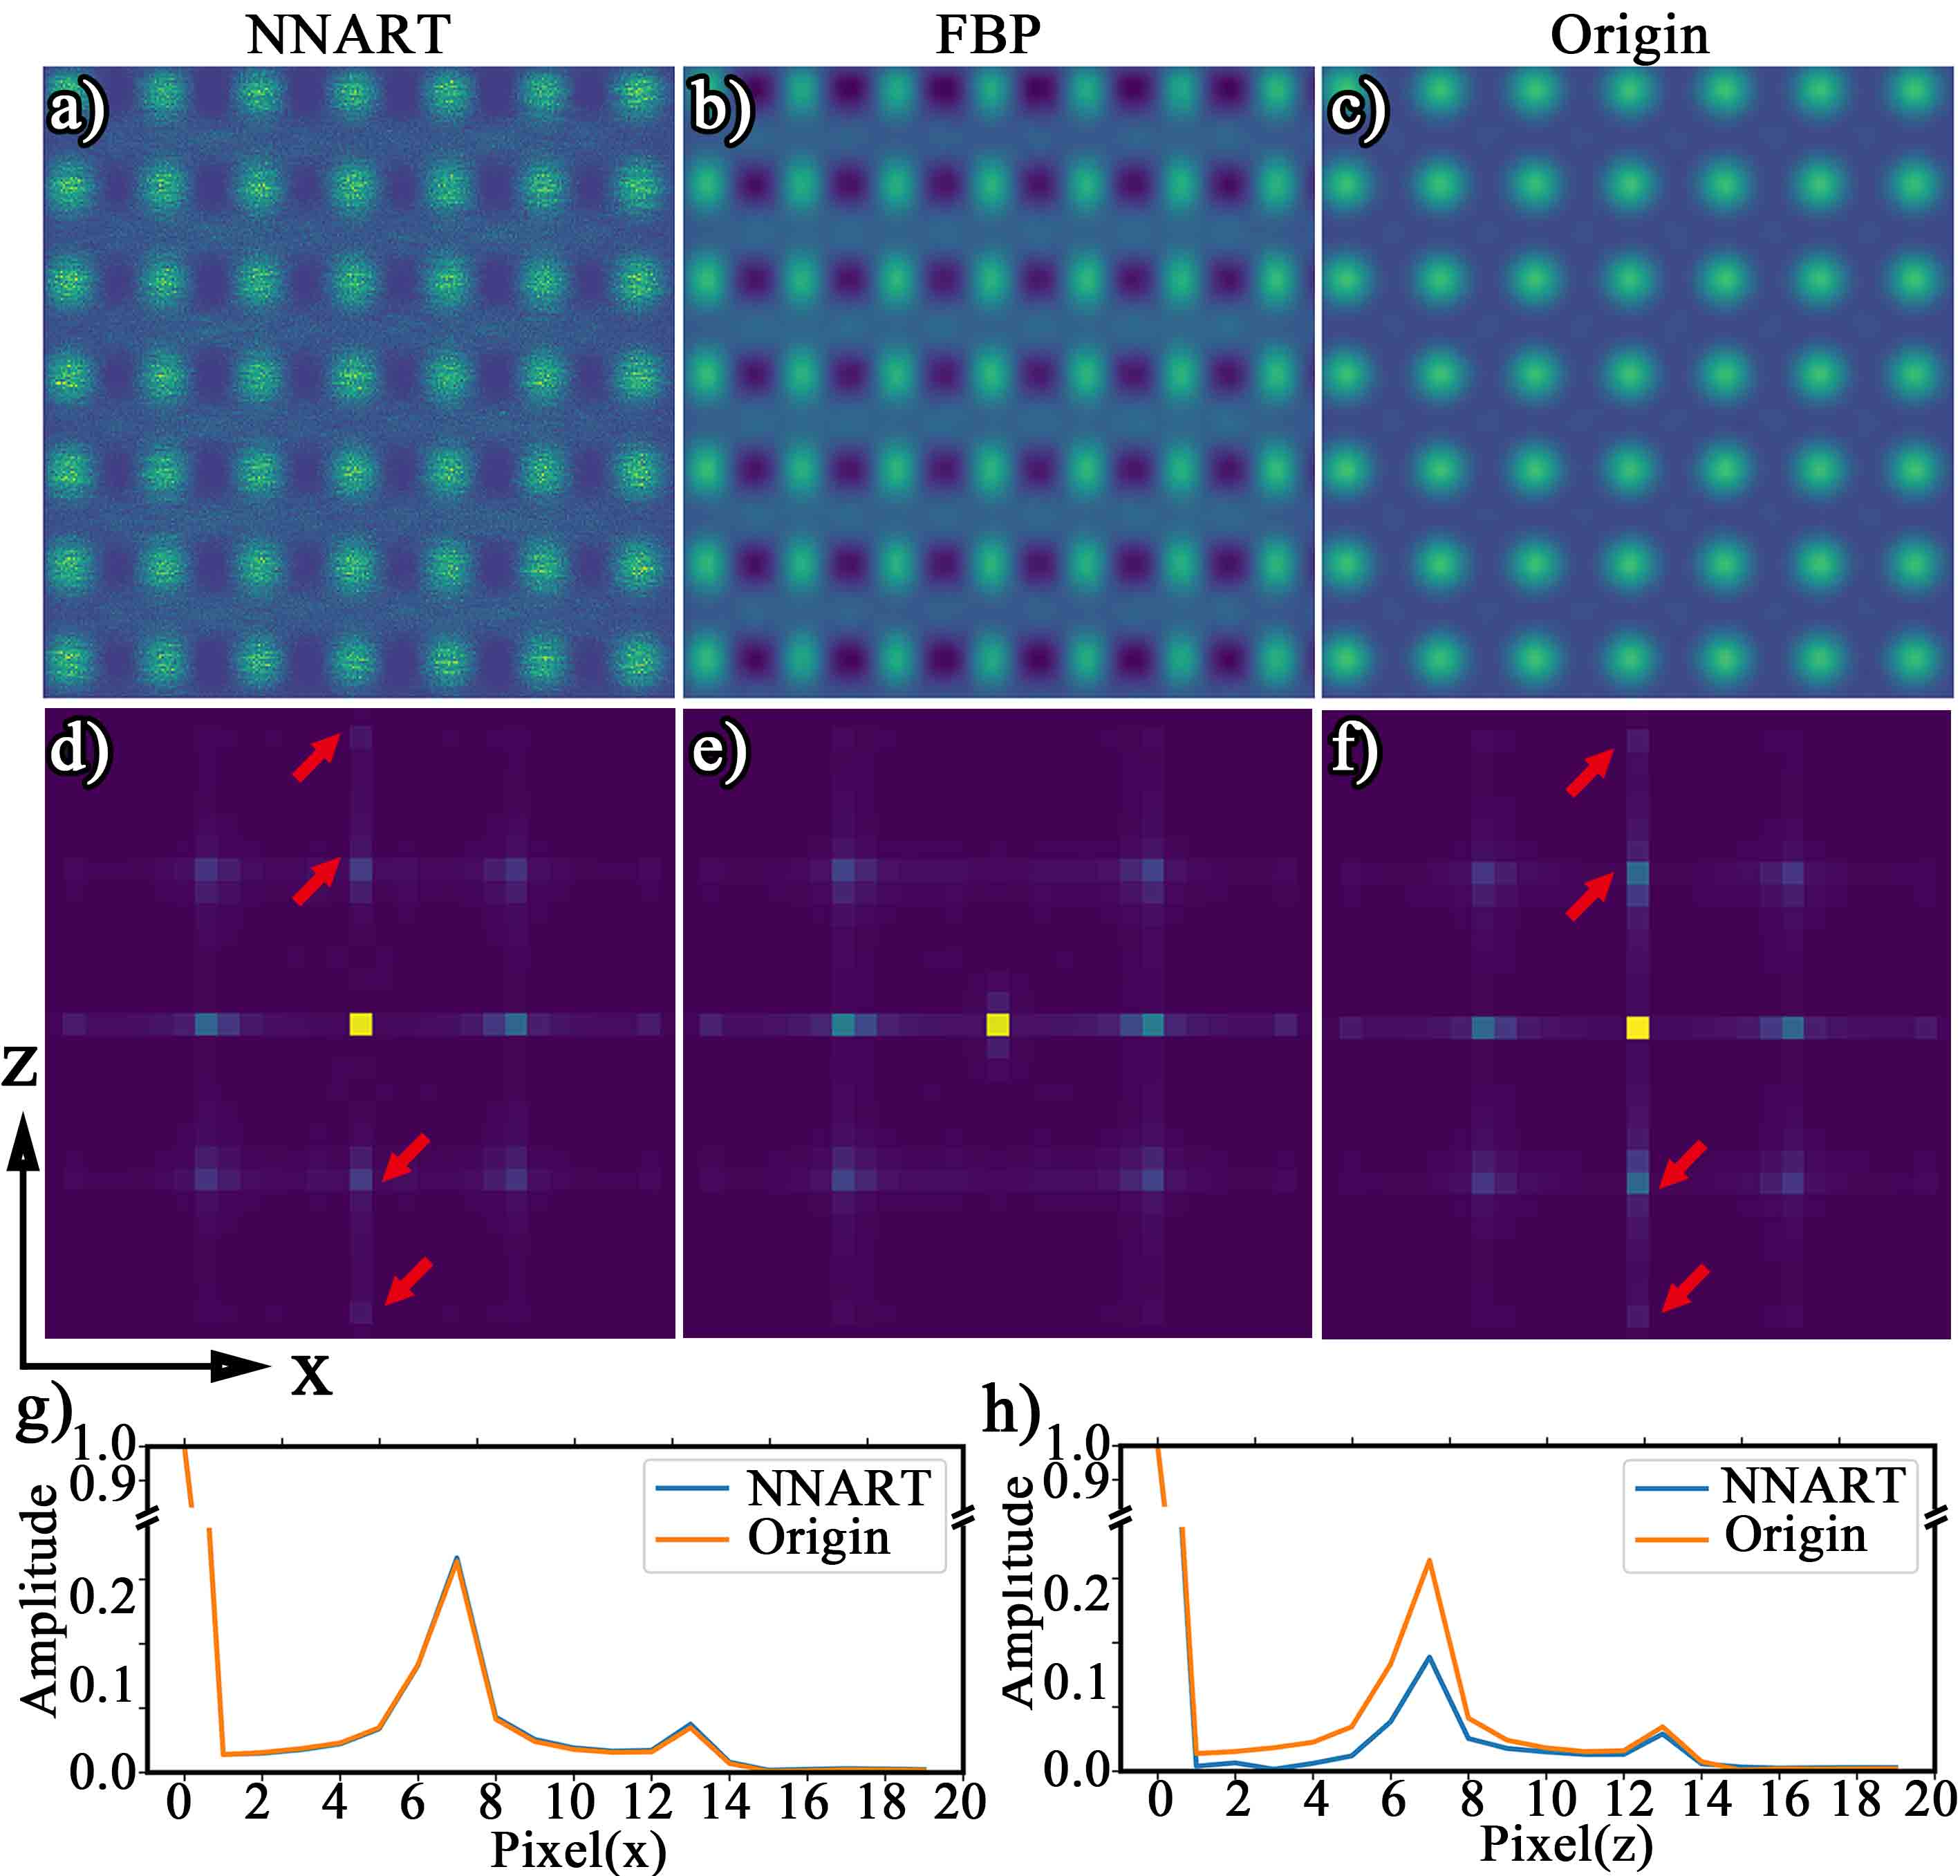
\includegraphics[width=0.9\textwidth]{../3.7/37}
	\caption{NNART 对 STEM 模拟原子像的重构测试}\label{fig:37}
	\song\tuzhu{a,b) NNART 和 FBP 重构 STEM 模拟原子像的带有缺失锥的 sinogram 的重构结果;c) STEM 模拟原子像;d,e,f) 图 a,b,c 的傅里叶变换(仅展示中间局部区域);g,h) 图 d 和 f 沿 $x$ 轴和 $z$ 轴的振幅对比曲线;sinogram 的倾转角范围是 -70° 至 +70°,倾转间隔是 1°}
\end{figure}

\section{实验及结果}
本节使用 NNART 重构了 SiC 样品,以验证 NNART 在实验数据中的适用性。SiC 样品是非晶转化法制备的纳米晶连续 SiC 纤维,制备工艺是将含铝的聚碳硅烷在 300 °C 的氮气保护下熔融纺丝、160  °C 空气中预氧化,随后在 1800 °C 氮气保护下热裂解。如图 2.11a 所示,样品是经离子束切割的 SiC 纤维的截面样品~\cite{Zhang2018},呈圆盘状且纵横比很大。样品在 FET Tecnai F20 透射电镜中,沿 $y$ 轴为倾转轴,以 -70° 至 +70°,1° 为间隔拍摄 HAADF-STEM 倾转系列像。本研究只重构了图 2.11a 中感兴趣区区域的部分。图 2.11b 展示了感兴趣区区域的倾转前(倾转角为 0°)的 HAADF-STEM 实验图像。其中石墨或游离炭由于 C 元素的原子序数很小,所以在 HAADF-STEM 像中呈暗衬度,如白色箭头所示。可见,这些石墨或游离碳没有固定的形状,它们不规则地分布在 SiC 基体中,形成了复杂的内部形貌。当样品倾转至 70° 时,可从图 2.11c 和 b 的对比看出,其 HAADF-STEM 的图像强度明显增强,这是因为在大倾转角下,样品沿 $z$ 轴的有效厚度增大导致的。图 2.11c 中最右侧的亮衬度物质是离子束切割过程中,样品表面沉积的重元素 Pt。另可知图 2.11b 所展示的感兴趣区,在图 2.11c 中仅为两条红色虚线内的区域。最后,在进行三维重构之前,所有的 141 张倾转系列 HAADF-STEM 图像都使用了互相关法进行了漂移矫正。

\begin{figure}[htbp]
	\vspace{\baselineskip}
	\centering
	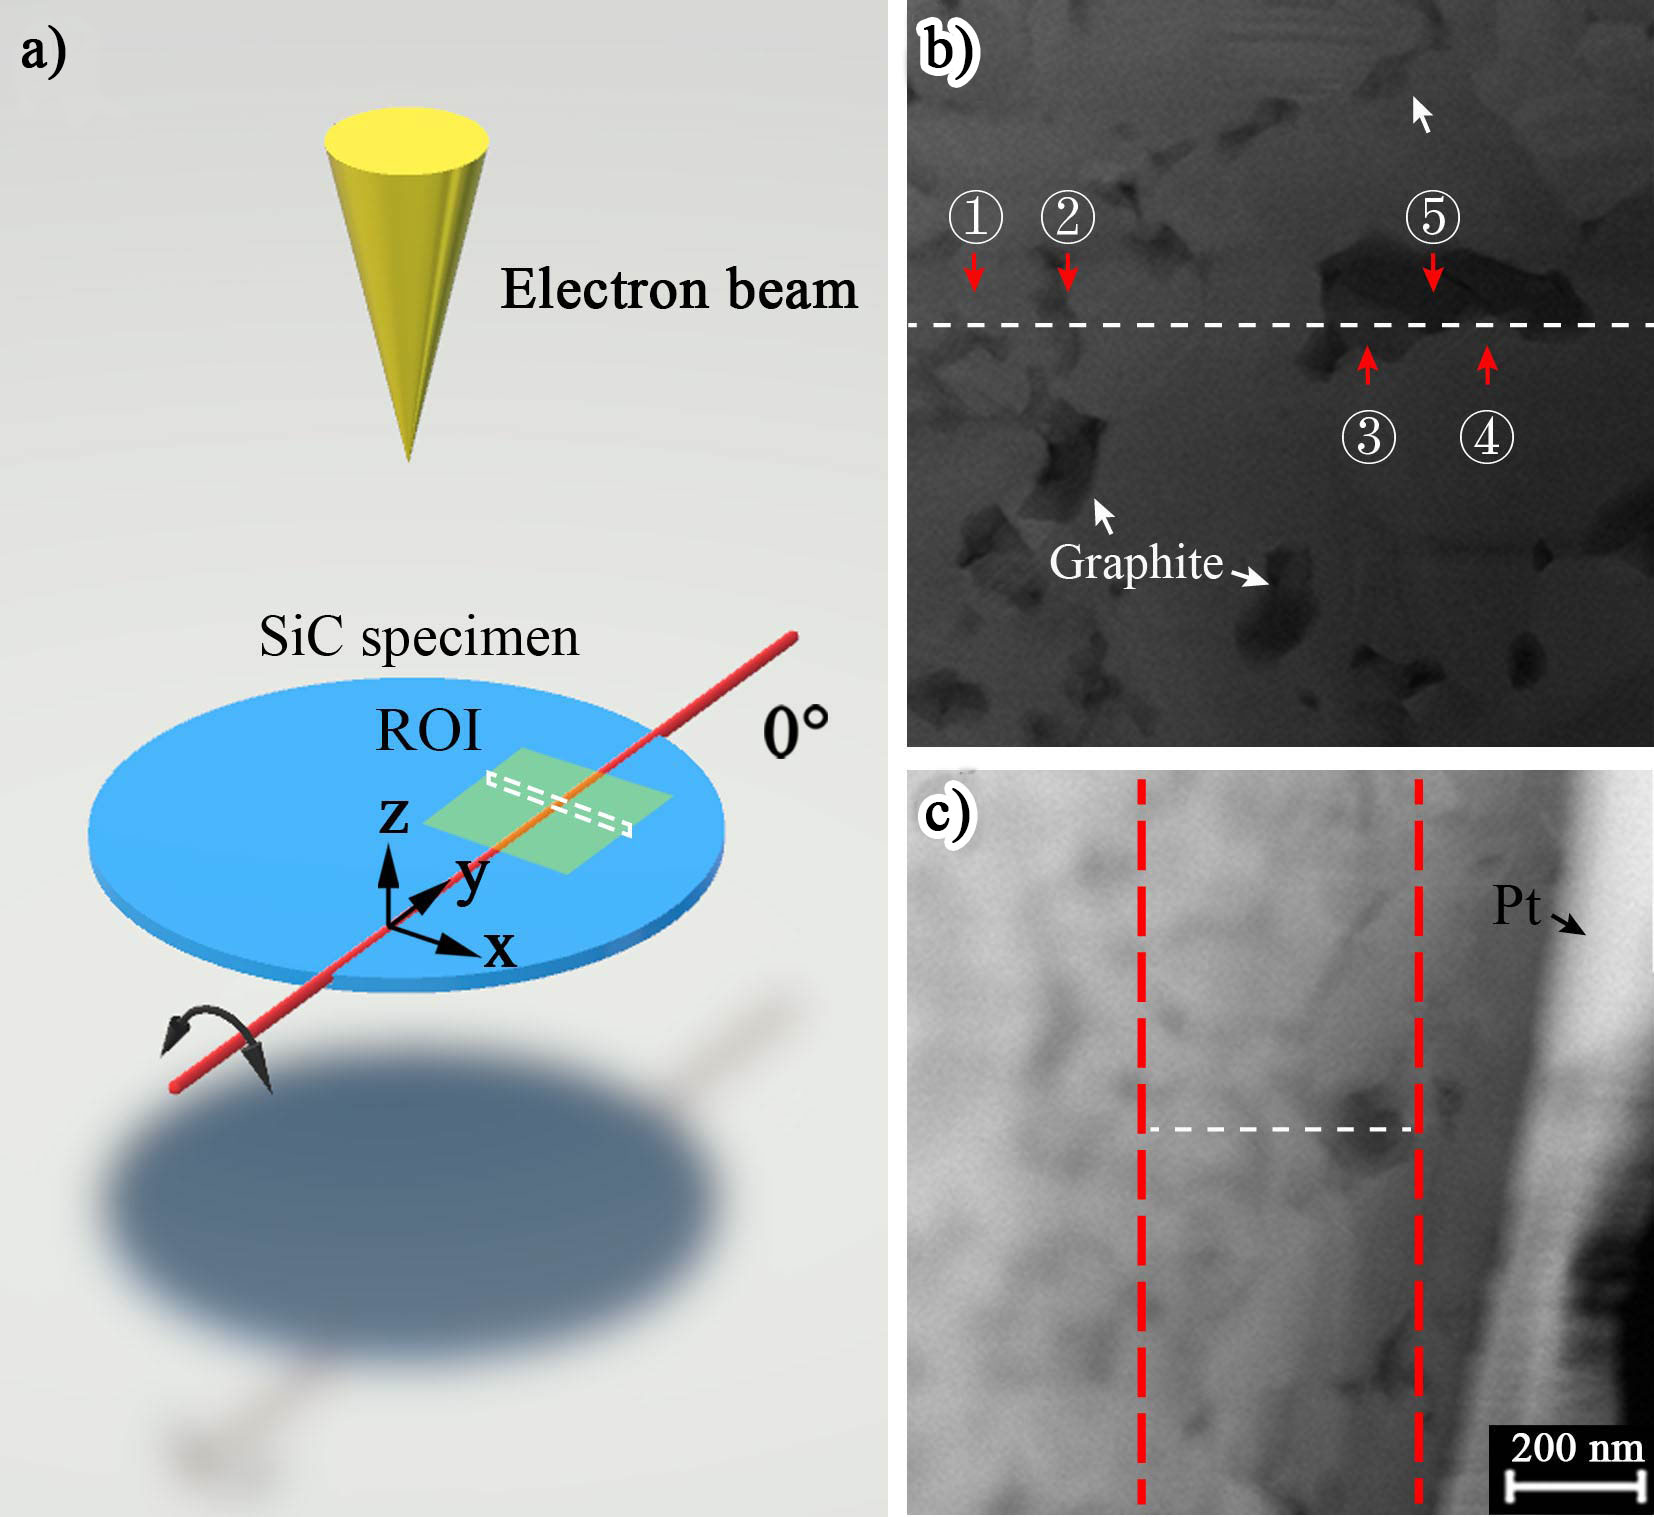
\includegraphics[width=0.9\textwidth]{../3.8/38}
	\caption{SiC 样品图示}\label{fig:38}
	\song\tuzhu{a) SiC 样品在 HAADF-STEM 倾转系列像实验中的布局示意图,电子入射方向沿z轴向下;b, c)SiC 分别倾转 0°(倾转前)和倾转 70° 时的 HAADF-STEM 实验像;图 b 的视野是感兴趣区,而其仅为图 c 中两条红色虚线之间的区域;图 a 中的白色虚线框和图 b 与 c 中的白色虚线表示了样品中某一片层,图 b 中标注的 5 个特征点有助于对重构结果的分析}
\end{figure}



 图 2.12a 和 c 展示了 NNART 和 TVM 重构的图 2.11b 中白色虚线处的一层 SiC 样品。图 2.12b 和 d 展示了图 2.12a 和 c 的傅里叶变换,显然 NNART 在傅里叶空间中恢复出了更多的缺失锥区域的信息,而 TVM\begin{figure}[b!]
 	\vspace{\baselineskip}
 	\centering
 	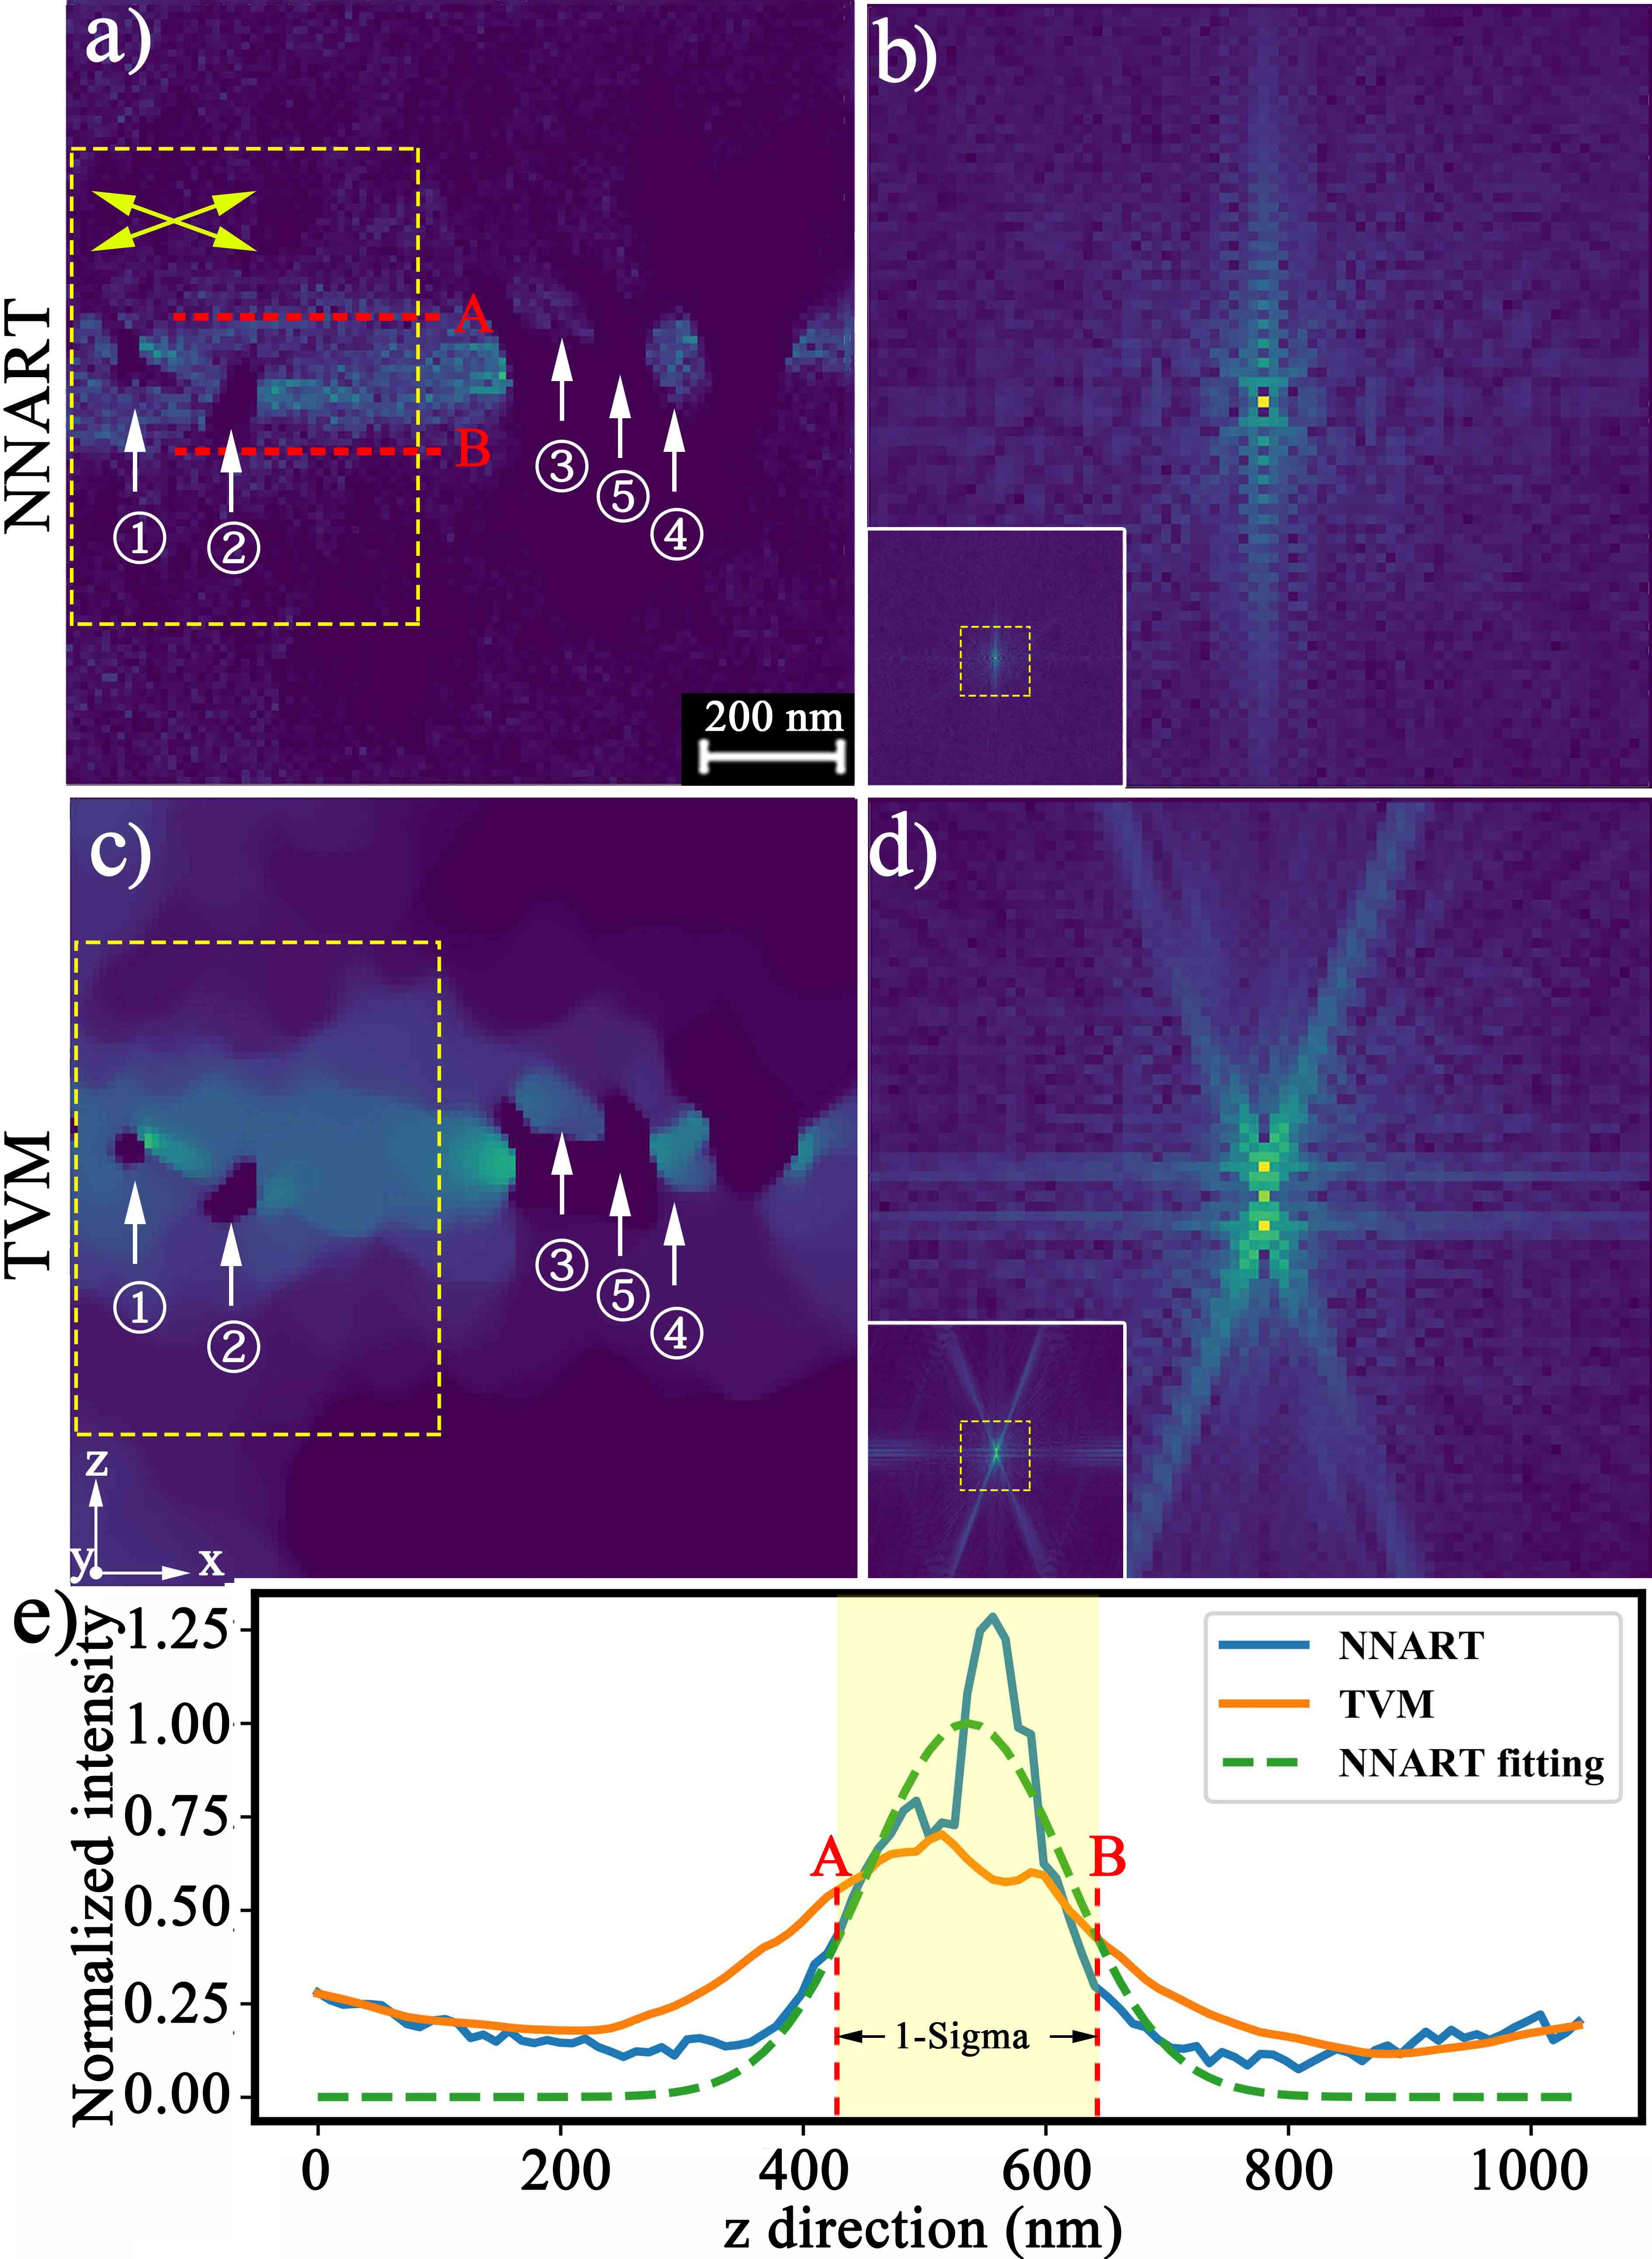
\includegraphics[width=0.65\textwidth]{../3.9/39}
 	\caption{NNART 和 TVM 重构的二维结果的对比}\label{fig:39}
 	\song\tuzhu{a, c) NNART 和 TVM 重构的图 2.8b 中白色虚线处的 SiC 样品,对应的 5 个特征同样用虚线标注;b, d) 图 a 和 c 的傅里叶变换(插入的小图)的中间放大图像;e) 图 a 和 c 中黄色虚线框中沿 $z$ 方向的归一化强度分布对比图,绿色虚线是蓝色实现的正态分布拟合曲线,其中红色虚线 A 和 B 与图 a 中的虚线位置对应,其中包括的是正态分布曲线的 1-Sigma 区域}
 \end{figure}仅在非常低频的位置恢复出了些许信息,整个信息缺失的锥形样貌在图 2.12d 中仍然非常明显。在这个实验案例中,TVM 对缺失信息的恢复比第 2.3 节中的模拟案例差很多,其原因是 TVM 将样品周围的噪音错误地加强了,这在图 2.12c 中表现得很明显。因此,TVM 重构的结果中的样品并不像离子束切割样品预期的那样边界笔直,很多被错误加强和平滑的噪音在其周围形成了不规则的形貌。而图 2.12a 中展现出的整体的样品形貌更加合理,尽管 NNART 无法去除来自实验数据的噪音。在两个算法的重构结果中,图 2.11b 中的特征 1、2、3、4 均得到了较为正确的还原,唯一不同的是图 2.11a 和 c 中恢复的特征 1 的形状并不相同,NNART 的重构结果是 $\lambda$ 形,这个结果经图 2.16i 和 j 可以验证,是正确的。而 TVM 的重构结果是一个小圆形,这是图像平滑处理的结果。所以 NNART 重构出了样品的更多细节。图 2.12e 是图 2.12a 和 c 中黄色虚线框中的图像强度沿 $z$ 方向的平均变化曲线。绿色的虚线是 NNART 测得的曲线的高斯分布拟合,其 1-Sigma 区域对应于图 2.12a 的 A、B 虚线,可见这是对样品厚度的合理测量。而 TVM 的曲线则宽很多,显然无法正确测量样品的厚度。
 
\begin{figure}[H]
	\vspace{\baselineskip}
	\centering
	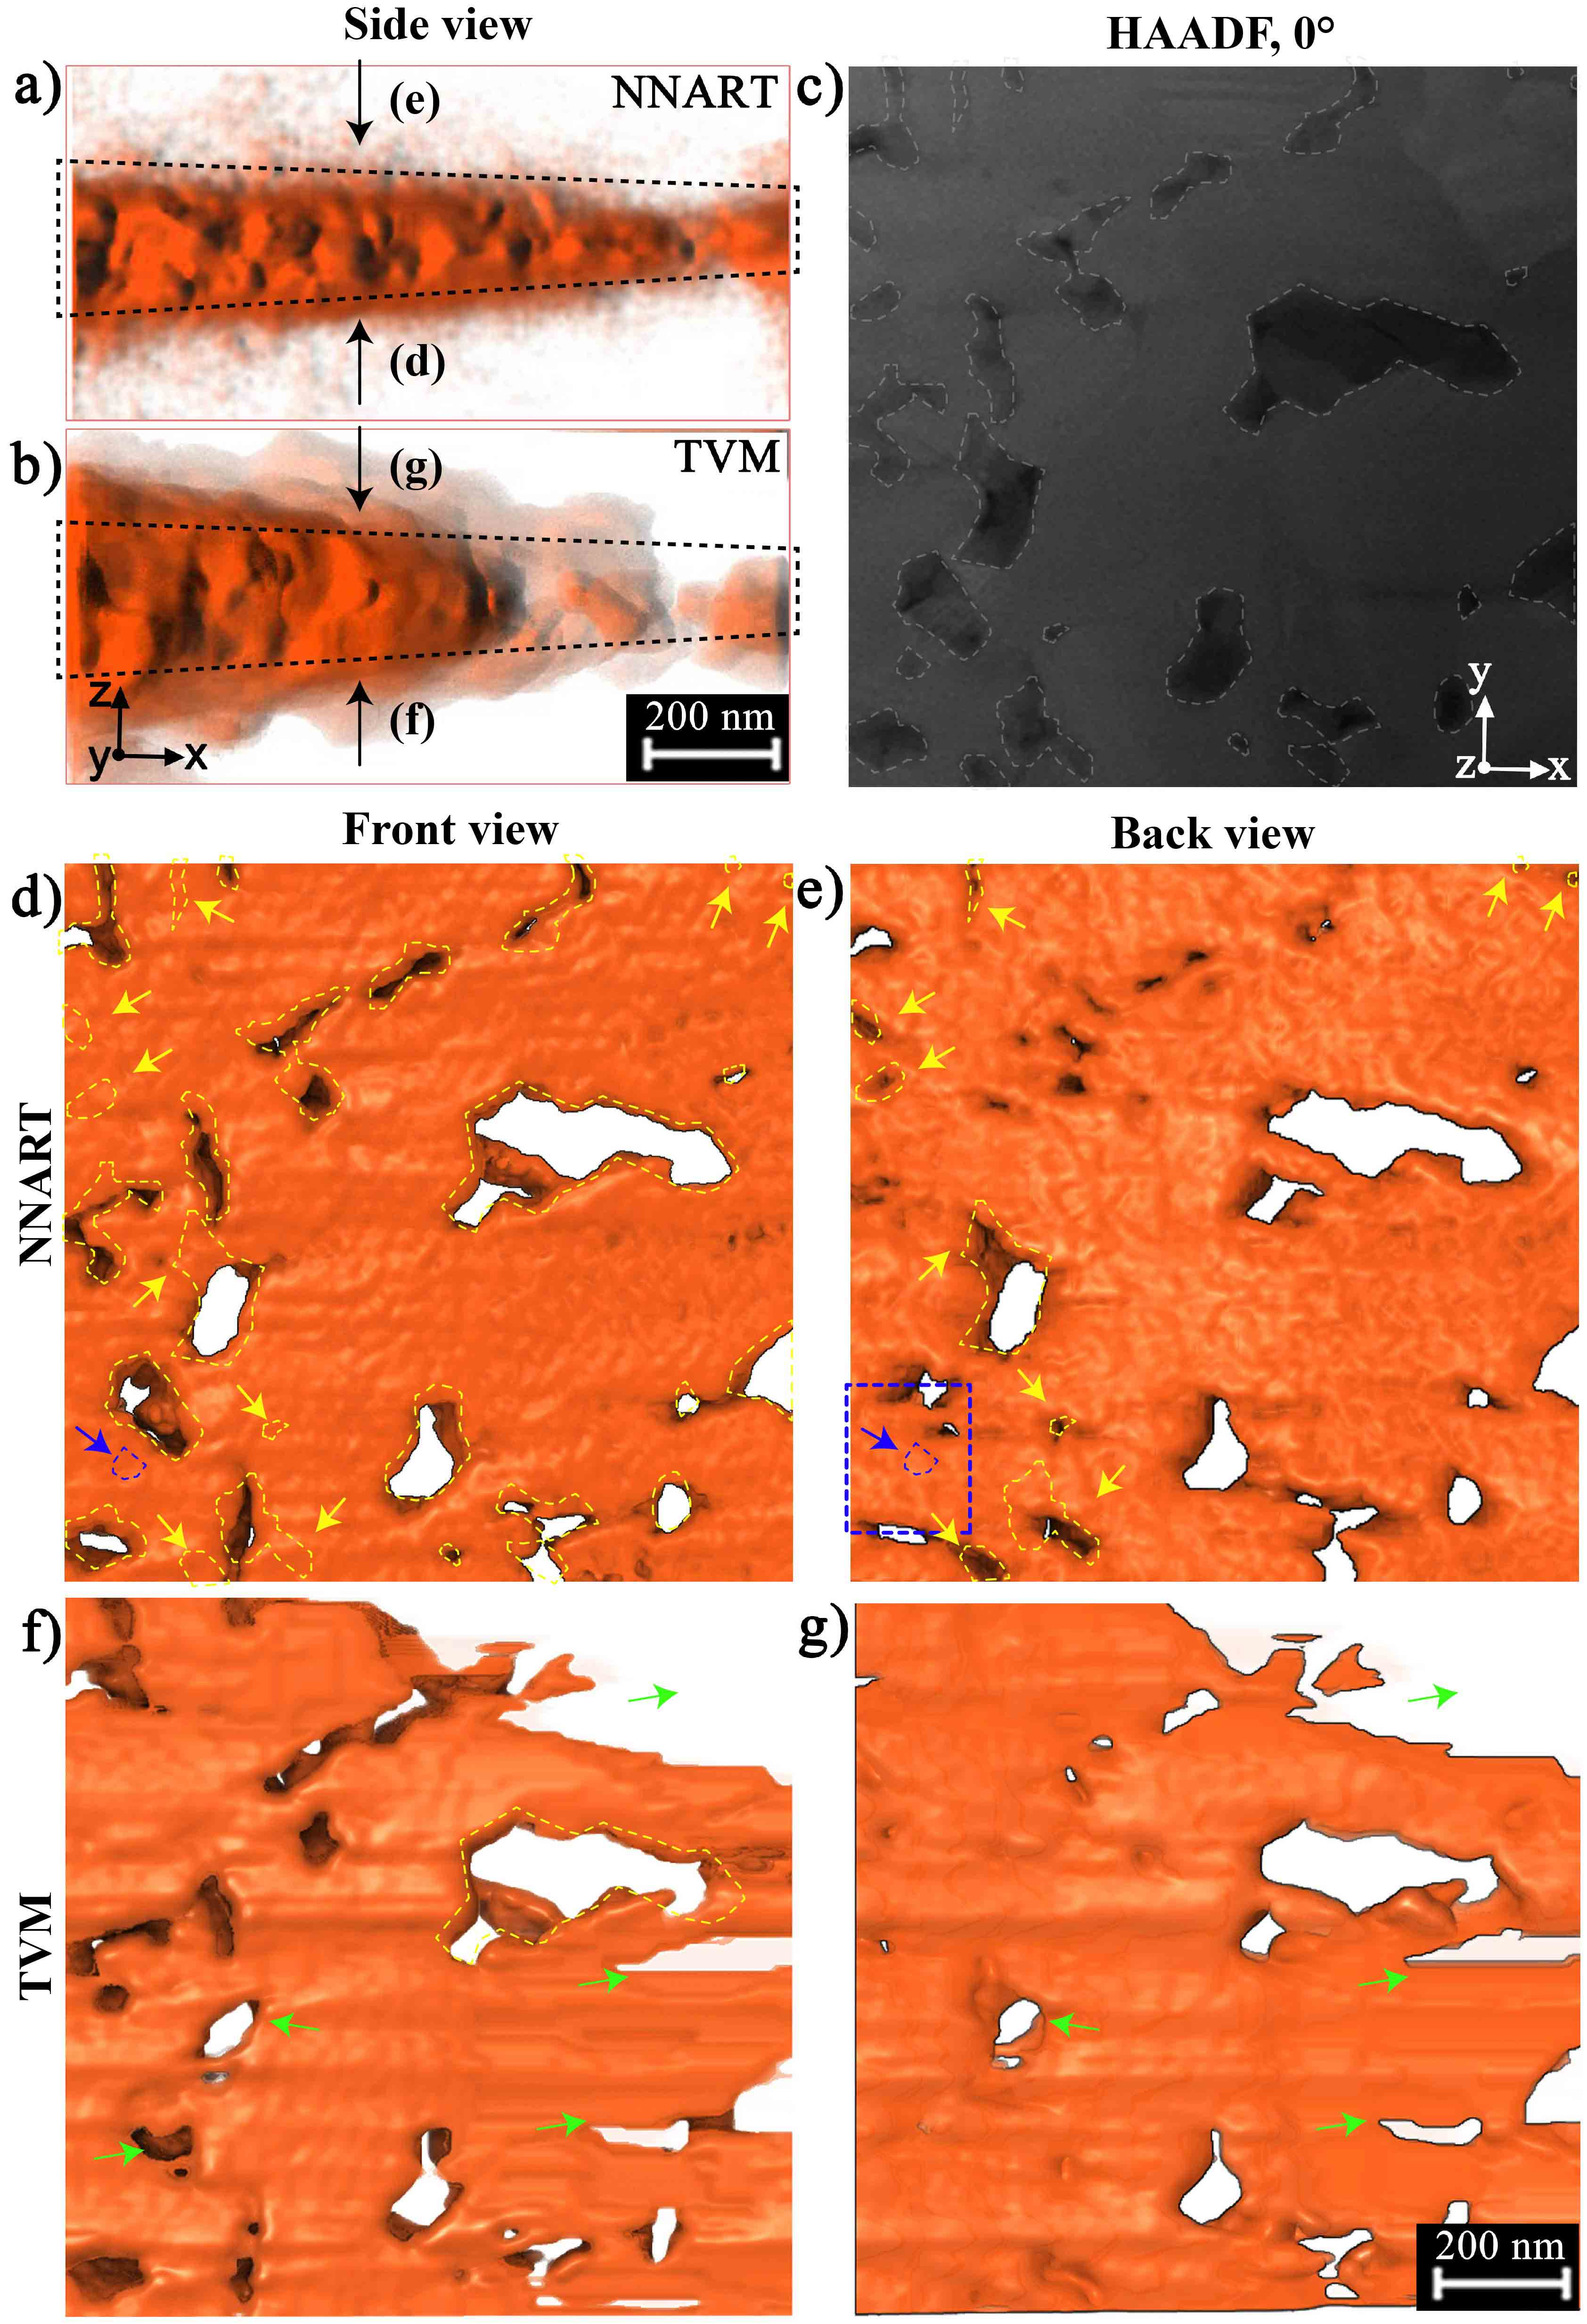
\includegraphics[width=0.65\textwidth]{../3.16/316}
	\caption{SiC 样品三维重构渲染图}\label{fig:310}
	\song\tuzhu{a,b) NNART 和 TVM 重构的 SiC 样品的俯视视角三维渲染图;c) 倾转角为 0° 时的  HAADF-STEM 实验图;d,e) 图 a 中虚线框内的重构结果的前视图和后视图;其中,图 d 中的虚线轮廓与图 c 中的一一对应,黄色箭头指出的形貌仅显示在图 e 中;蓝色虚线框处被剖开后可观察到蓝色箭头所指的相;f,g) 图 b 中虚线框内的重构结果的前视图和后视图;绿色箭头所指的形貌明显偏离图 c}
\end{figure}

图 2.13a 和 b 展示了 NNART 和 TVM 重构的 SiC 样品的三维渲染结果的俯视图(与图 2.12a 和 b 相同视角)。图 2.13a 清晰地展示出了一个具有厚度梯度的片状(离子束切割)样品的形貌,纵横比约等于 5。而图 2.13b 中 TVM 重构的结果并不理想,样品呈现出许多不规则的形貌,不符合离子束切割样品的形貌。为了进一步观察重构的样品的形貌,图 2.13d 和 e 展示了图 2.13a 中虚线框内部分的前视图和后视图。图 2.13c 和 d 中的虚线轮廓是一一对应的,通过对比可见石墨和游离碳相由于衬度较弱,显示为孔洞状,且图 2.13d 中能够观察到绝大部分的石墨和游离碳,形貌与实验图像吻合。少部分黄色箭头所指的相,在前视图中无法观察到,因为它们实际存在于背面,可在图 2.13e 中观察到。蓝色箭头与轮廓所指的相,存在于基体的内部,在图 2.13d 和 e 中均无法观察到。图 2.14 展示了将图 2.13e 中蓝色虚线框内的部分剖开后,不同深度处的样品形貌,可见该相存在于 $z \approx 65 \sim 135$ nm 的深度内。图 2.13f 和 g 展示的是图 2.13b 中虚线框内部分的前视图与后视图。可见,TVM 重构的形貌与实验图像相去甚远,仅黄色虚线轮廓中的大的石墨相得到了较好的重构,绿色箭头处还出现了严重的错误。综上可知,NNART 在重构该 SiC 样品时,具有非常大的优势,它的重构结果较为准确。






\begin{figure}[htbp]
	\vspace{\baselineskip}
	\centering
	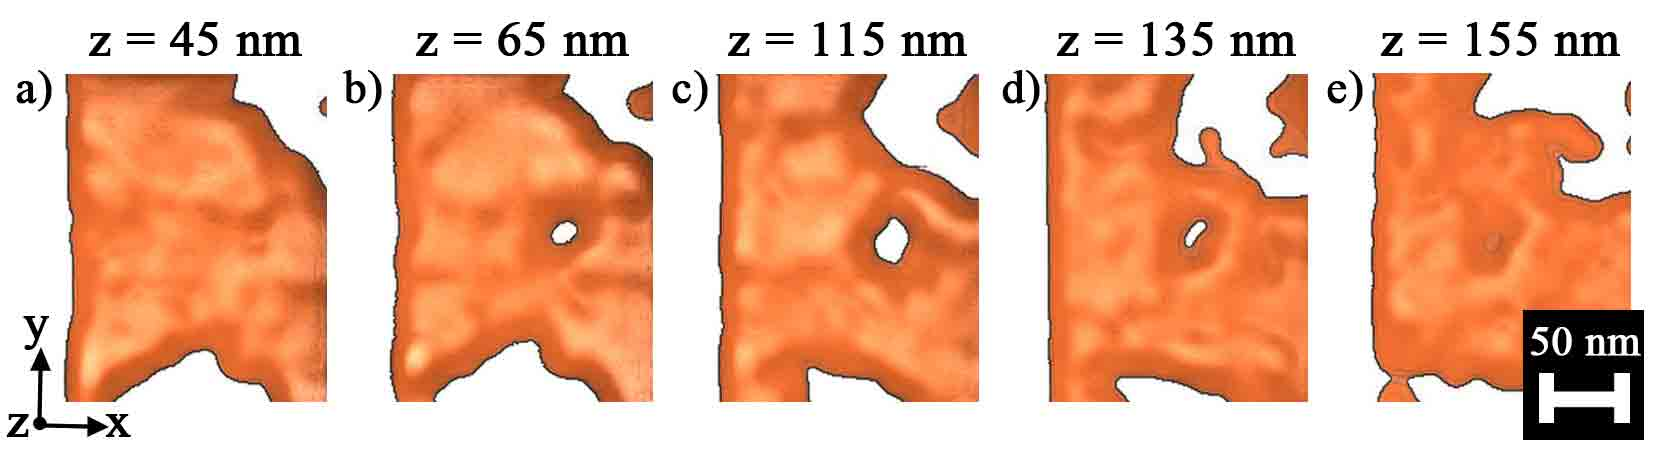
\includegraphics[width=0.9\textwidth]{../3.18/318}
	\caption{SiC 样品三维重构局部的切片渲染图}\label{fig:310}
	\song\tuzhu{a-e) 图 2.13e 中蓝色虚线框中部分在不同深度下的切片的渲染图,深度 $z$ 分别为 45、65、115、135 和 155 nm}
\end{figure}

为了进一步在三维的维度上说明 NNART 重构的样品形貌的准确性,图 2.15 对比了不同倾转角下的石墨相的的三维重构渲染图与实验图。可见在任意角度下,石墨相的三维渲染图展示的形貌与实验图像都非常相近,这说明这个石墨相的三维形貌被准确地重构了出来。由此可知 NNART 重构的样品形貌是相当准确的。
\begin{figure}[htbp]
	\vspace{\baselineskip}
	\centering
	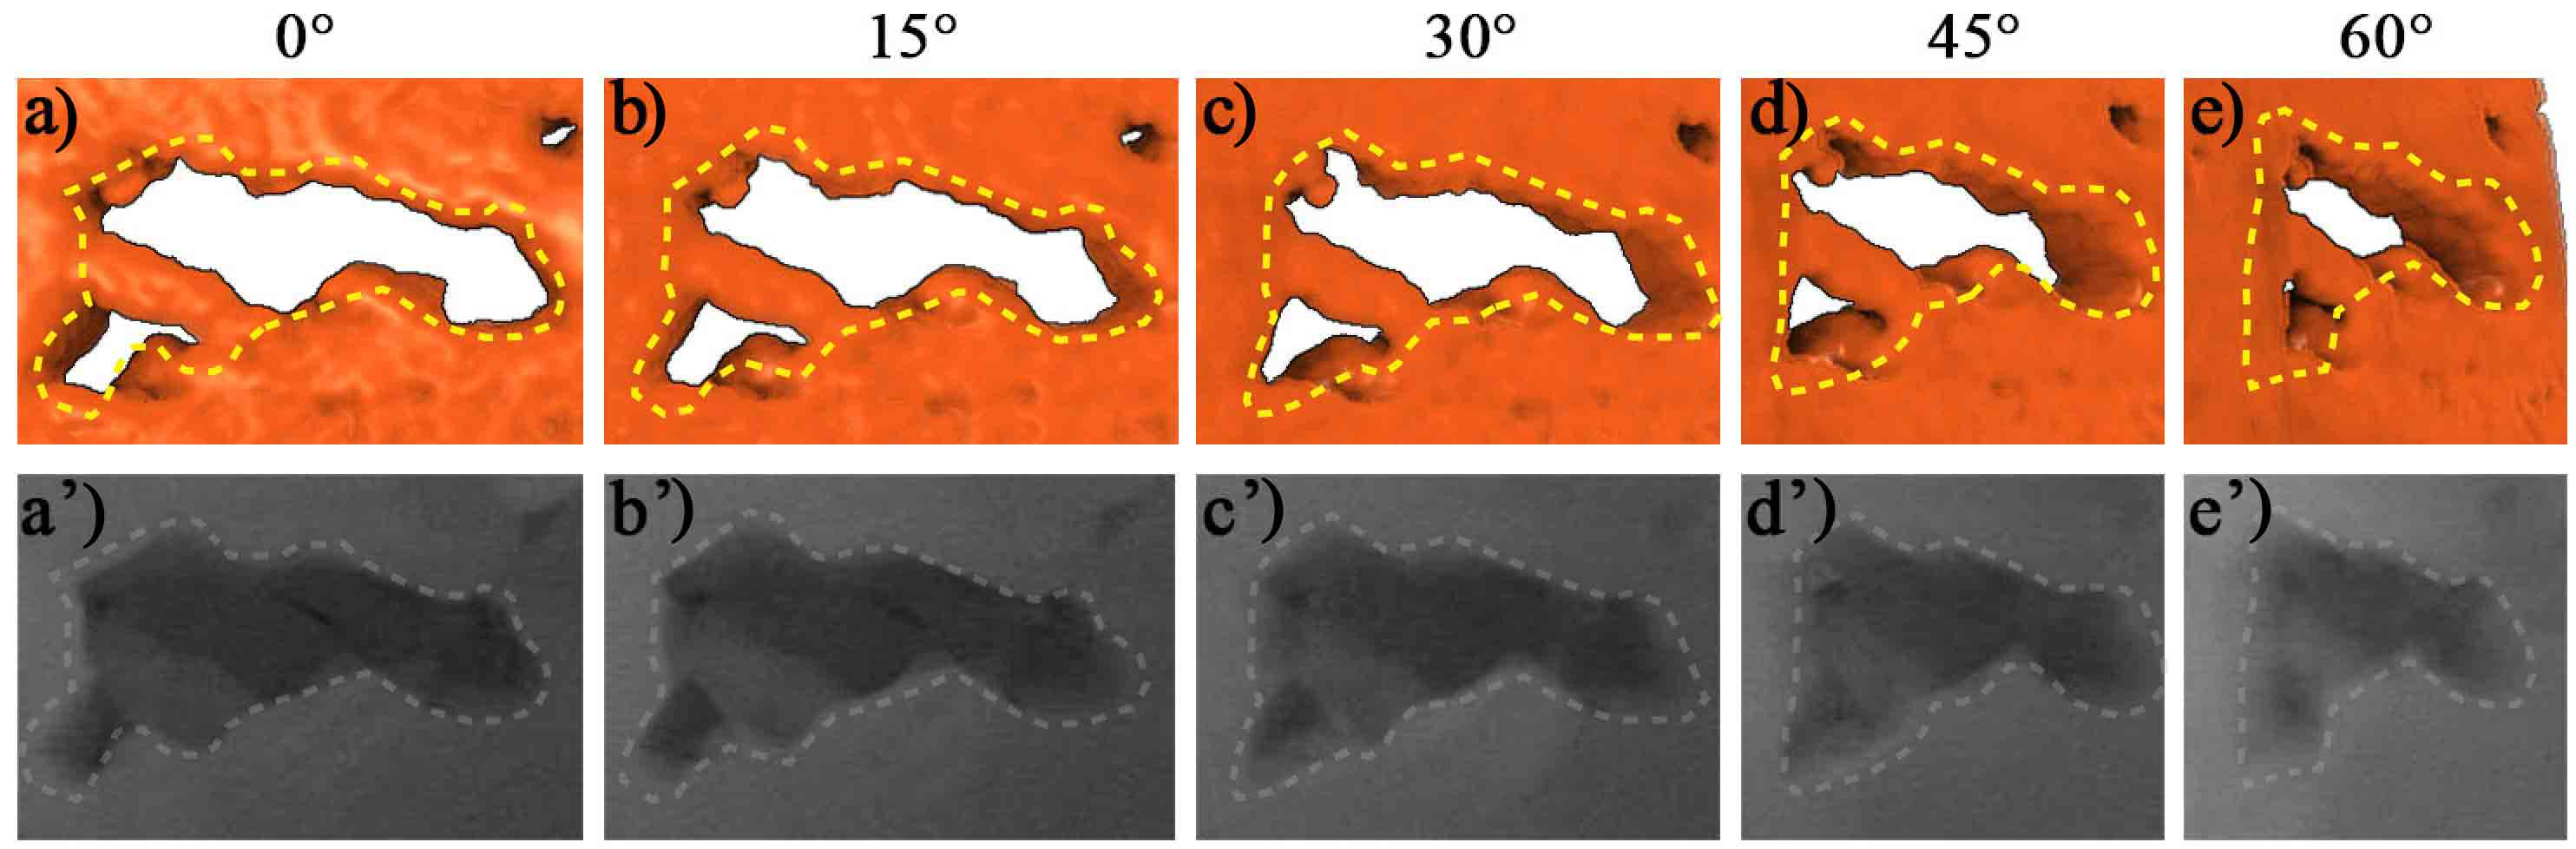
\includegraphics[width=0.9\textwidth]{../3.17/317}
	\caption{石墨相在不同倾转角下的三维渲染图与实验图像的对比}\label{fig:310}
	\song\tuzhu{a-e) NNART 重构的石墨相分别在 0°,15°,30°,45°,60° 倾转角下的三维渲染图;a'-e')  0°,15°,30°,45°,60° 倾转角下的石墨相的实验图}
\end{figure}

\section{NNART 与正则化}
本节将探究 NNART 的正则化,具体实施方法为在公式(2.6)的损失 $L$ 中加上一个正则化项:
\begin{equation}
L = \sum {\sqrt{|\boldsymbol{S}-\boldsymbol{S}^{exp}|}}+\alpha V
\end{equation}
其中 $\alpha$ 是正则化系数,$V$ 是正则化项。由于正则化的算法可以得到平滑解,所以在此不再需要使用“多次平均”,正则化后的 NNART 每次只需重构一次即可得到重构结果。研究中使用的正则化方法有 L2 范数、最大熵(香农熵)以及 TVM,其中 L2 和香农熵的正则化项分别为:
\begin{equation}
V_{\text{L2}} = \sum \boldsymbol{I}^2
\end{equation}
\begin{equation}
V_{\text{Shannon}} = -\sum \boldsymbol{I} \log_2 \boldsymbol{I}
\end{equation}

\begin{figure}[htbp]
	\vspace{\baselineskip}
	\centering
	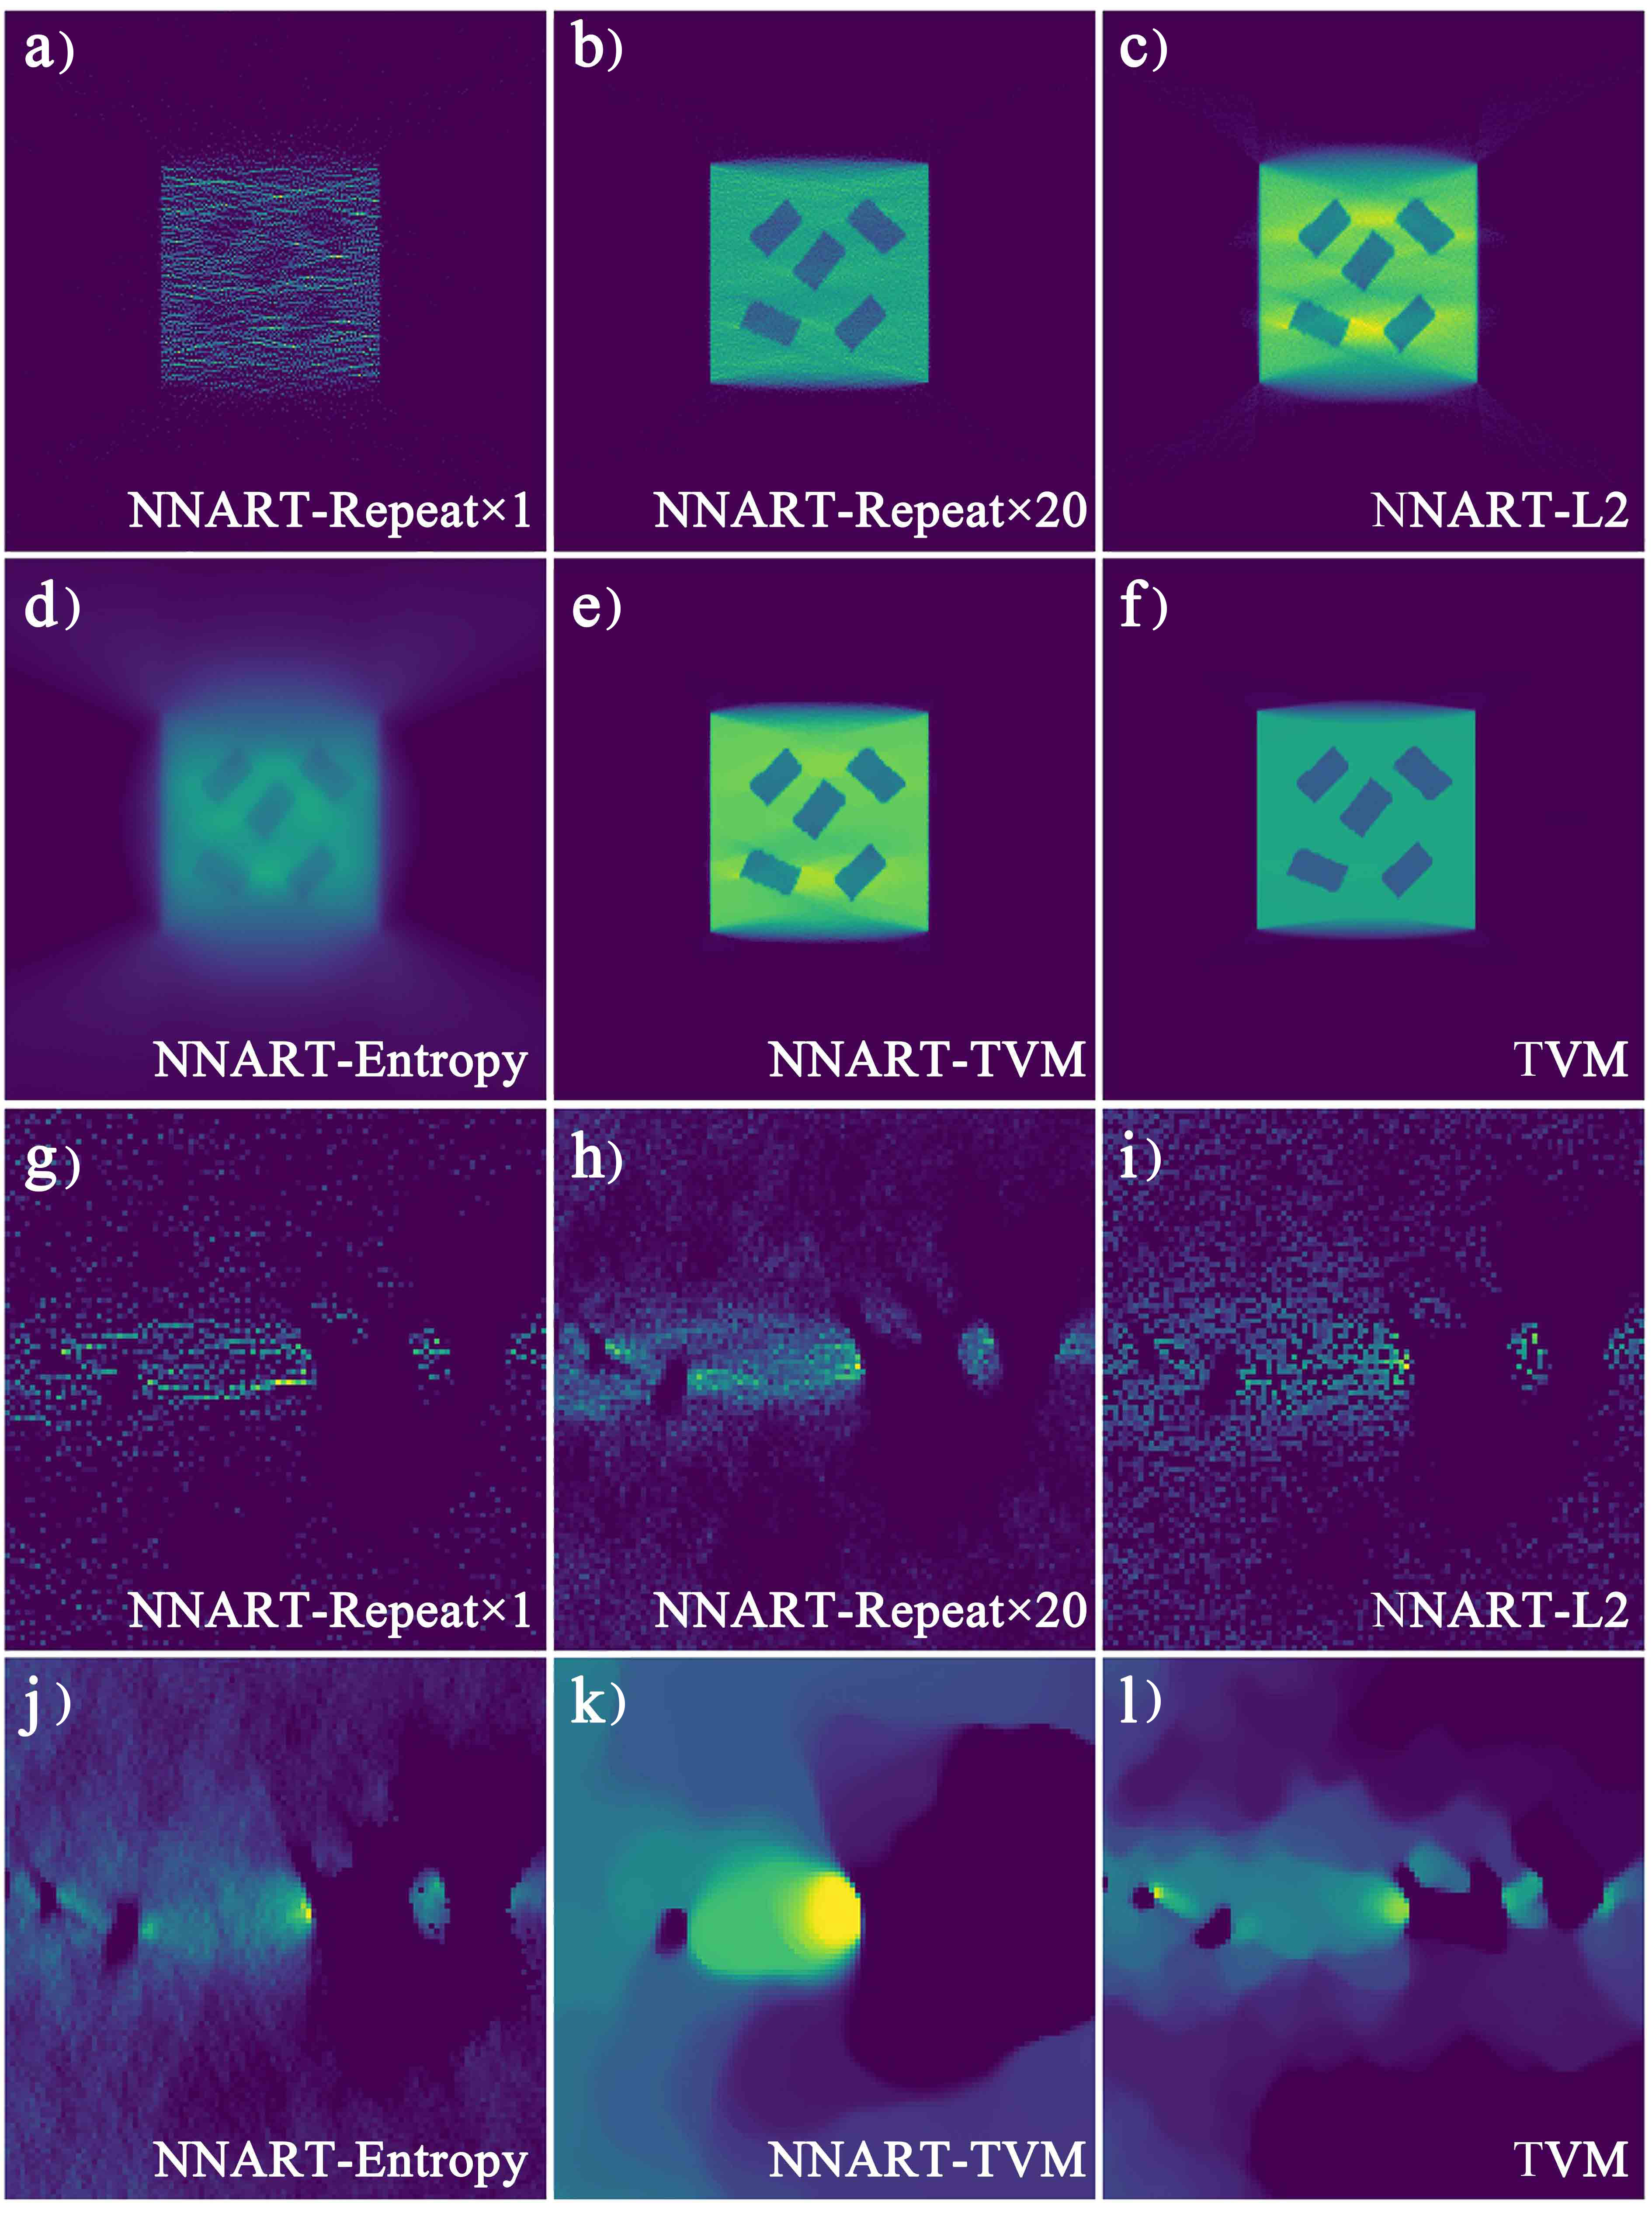
\includegraphics[width=1.0\textwidth]{../3.11/311}
	\caption{NNART 正则化与非正则化下的重构结果对比}\label{fig:311}
	\song\tuzhu{a-f) NNART 一次重构、20 次重构平均、L2 正则化、最大熵正则化、TVM 正则化以及 TVM 算法的模型 1 的重构结果;g-l) NNART 一次重构、20 次重构平均、L2 正则化、最大熵正则化、TVM 正则化以及 TVM 算法的 SiC 片层的重构结果}
\end{figure}

图 2.16 以模型 1 以及图 2.12 中使用的 SiC 样品中的某一层为例,对比了 NNART 在仅重构一次、取 20 次重构平均以及不同正则化项下的重构结果。图 2.16a 和 g 是 NNART 一次重构的结果,如第 2.3.1 条所述,该结果中存在非常严重的噪音。而如图 2.16c-e 所示,在 NNART 经过正则化后,仅需一次重构就能得到平滑解。与图 2.16b 和 f 对比可知,对于模型 1 这种形貌较为简单,投影数据理想的情形而言,NNART 在 L2 和 TVM 正则化下,都具有一定的抑制缺失锥假象的作用,不过 L2 的效果稍差。而 NNART 在最大熵正则化后,虽然能够获得平滑解,但是缺失锥假象的抑制作用完全丧失,其重构结果基本与传统算法 WBP、SIRT 等的结果无异。当使用正则化后的 NNART 重构 SiC 的实验数据时,重构结果则没有如此理想。图 2.16i 展示了 L2 正则化下的 NNART 重构结果,无论如何调节算法的学习率和正则化因子,重构结果中总是会出现严重的椒噪音,所以这种方法基本无法用来处理实验数据。而最大熵正则化下的重构结果(如图 2.16j 所示)则与模型 1 的重构情形一致,缺失锥假象没有得到任何抑制。图 2.16k 则是 NNART 在 TVM 正则化下的重构结果,该结果基本丧失了样品的细节。无论如何调节重构的参数,TVM 正则化后的 NNART 均无法很好地重构该实验数据,甚至在学习率偏大时会出现与图 2.16i 一样的椒噪音。



在 NNART 算法中,存在的较大的问题就是如何获得平滑解。正则化和“多次平均”是两种不同的解决问题的思路。正则化方法的优点是速度快,因为使用正则化后仅需一次重构就能得到平滑解。正则化在许多问题中均具有广泛的应用,同样地,在 NNART 算法中,当问题较简单时,正则化方法可以又快又好地得到平滑的、抑制了假象的重构结果。但是在 SiC 实验数据中,它无法很好地进行重构。所以,多次重构平均是更保险的一种选择。



当样品形貌较为简单时,正则化的 NNART 也能够获得不错的重构结果。图 2.17 展示了铝合金中析出相的 FBP、NNART 最大熵正则化、TVM 正则化的重构结果。图 2.17a-c 是三个重构结果的三维渲染图,从图中可以看出,析出相的形状尽管各不相同,但是都呈颗粒状,这种情况下缺失锥造成的假象相对较弱,重构难度不大。而这三种方法重构的结果基本一致,不过在一些颗粒的局部区域,如三图中的蓝色箭头所指处,FBP 的重构结果中衬度弱或不均匀,而这种现象在其他两个重构结果中得到了改善。图 2.17d-f 展示了图 2.17a-c 中黑色虚线处片层的二维重构图像。在图像的中间有一个体积较大的析出相,并且该析出相的纵横比相对较大,在图 2.17d 中可见析出相的上边界并不清晰,存在较严重的缺失锥假象。而在图 2.17e、h 中,该析出相的边界和周围的噪音分离,其形状较为清晰,所以缺失锥假象在一定程度上被抑制了。



该结果证明,在一般的纳米颗粒的重构中,NNART 的正则化方法也是一种良好的 3DET 替代方案。尽管神经网络的运算需要消耗一定的算力,但是在现代的计算机设备的运算能力下,不使用多次重构平均的 NNART 算法能够符合一般的应用需求。

\begin{figure}[htbp]
	\vspace{\baselineskip}
	\centering
	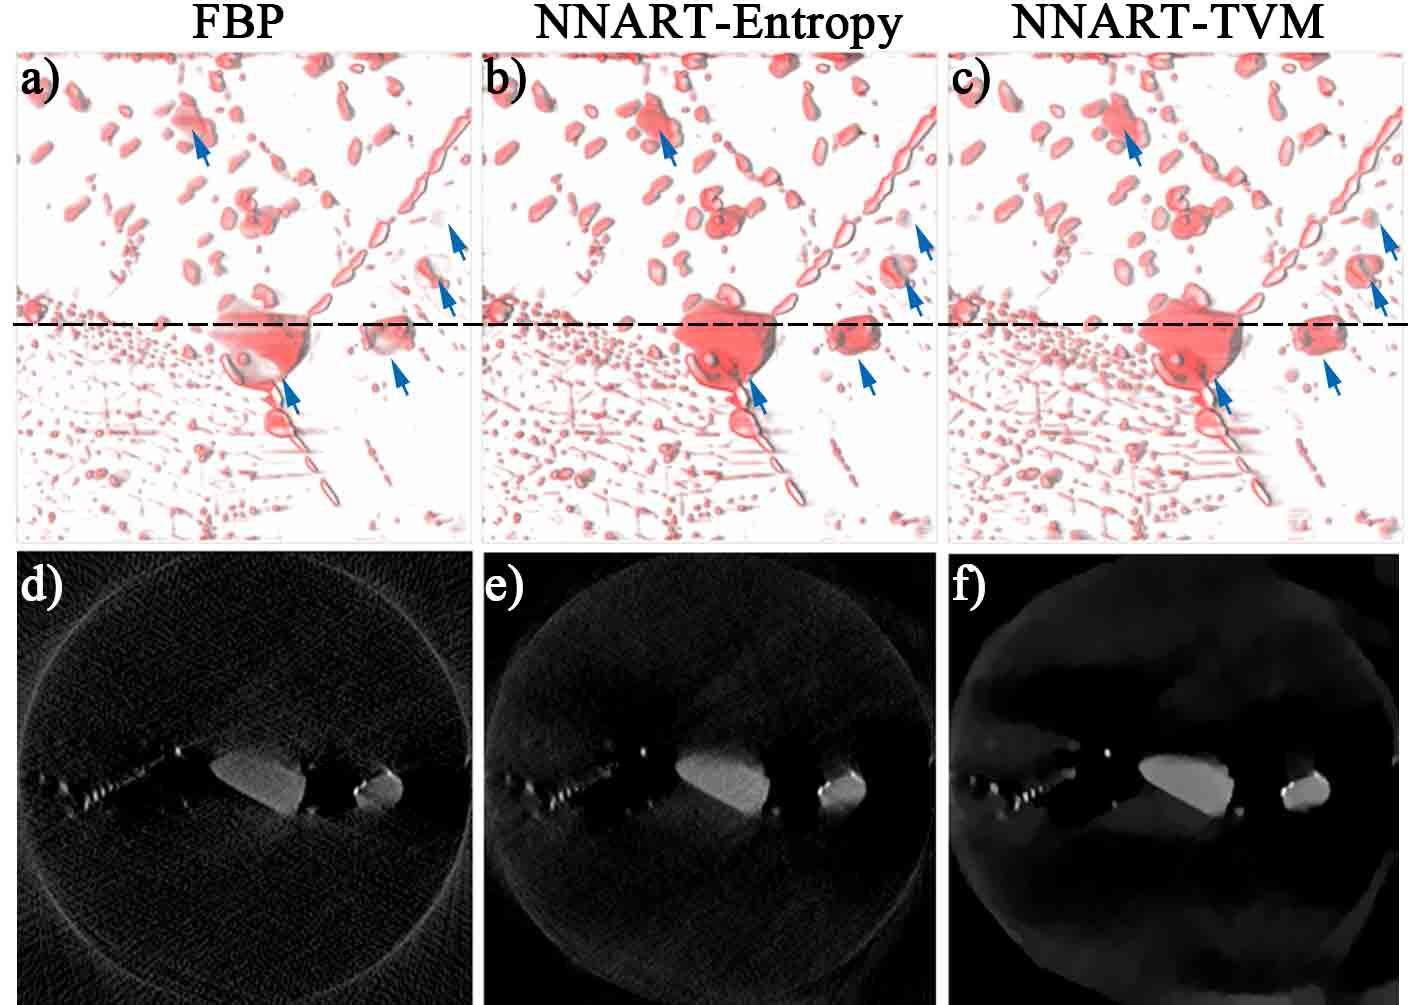
\includegraphics[width=0.85\textwidth]{../3.12/312}
	\caption{FBP、NNART 最大熵和 TVM 正则化重构铝合金析出相的结果对比}\label{fig:312}
	\song\tuzhu{a-c) FBP、NNART 最大熵和 TVM 正则化重构铝合金析出相的三维渲染图;d-f) 图 a、b、c 中黑色虚线处对应的片层的重构结果}
\end{figure}

\section{讨论}

\subsection{重构的精度与速度}
本章的研究内容主要围绕 NNART 抑制缺失锥假象这个主题。本节将简要论述 NNART 与其他主流三维重构算法的速度与精度,主要以 FBP、SIRT、TVM、DART 和 NNART 为例。其中,FBP 属于解析算法,是最简单的算法,SIRT 是 ART 等代数法的代表。而 TVM 和 DART 是典型的基于 SIRT 等迭代算法的约束或正则化方法。

这些方法运算速度的差异较大。对于重构一张 256 像素 $\times$ 256 像素的图像而言,在相同的计算机硬件条件下(比如因特尔 i7 系列的台式机中央处理器),FBP 能够在瞬间完成重构。SIRT、TVM、DART 的重构时间与具体参数选择有
很大关系,但一般在 1$\sim$10 分钟内可以完成重构,不过算法的复杂度是依次升高的。NNART 则需要更久的时间。不过,目前主流的计算机设备都配备有图形处理器。使用图形处理器加速,NNART 一般可以在 2 分钟以内完成一张 256 像素 $\times$ 256 像素图形的重构(一次重构)。真正制约 NNART 运算速度的是“多次平均”,尽管这些“多次”重构之间是相互独立的,可以同时进行,但这并不经济。

理论上,FBP 等解析法的滤波器(filter)只是对点扩散函数解卷积的近似,只有在具备足够多的全角度投影的情况下能够得到精确的重构结果。相同条件下,SIRT 的重构精度更高,当然这是用消耗更多运算资源所换取的。TVM 和 DART 等约束方法针对具有特定性质的材料提出,当重构对象符合这些算法的先验知识时,能够取得很好的重构结果,否则重构结果可能是错误的。而“多次平均”的 NNART 算法摒弃了这些先验知识条件,所以在应用上不受限制,当然其高精度的重构也是通过消耗更多运算资源得到的。不过,在图 2.5 的案例中,也发现 NNART 在某些情况下会出现过拟合现象,影响重构结果的强度分布。总体而言,更高的重构精度需要通过消耗更多的计算资源来实现。并且,讨论重构的精度时必须结合具体应用案例,比如对于原子分辨率的三维重构而言,重构的目标是原子的位置而非形貌,而更广泛的块体材料的三维重构的应用一般仅分析材料的三维形貌。真正重构材料物理性质的三维强度分布的应用案例(比如图 2.9 中的强度梯度)是罕见的。清楚地区分“物理精度”与“数学精度”是做好研究的基础。

\subsection{算法的优势与应用}
非线性神经网络能够对任何函数进行建模。当与反传播技术结合使用时,它可以建立实验投影数据与目标物体之间的关系。在重建过程中,可以从有效的实验数据中推断出缺失锥中丢失的信息。在简单的情况下(例如,图 2.5a),NNART 与正则化迭代方法相比没有明显的优势,因为此时正则化项与实际情况非常吻合。但在如 SiC 实验案例中,样品的实际情况因过于复杂而无法被编码为正则项时,NNART 的优势才会凸显。
NNART 的一种潜在应用是重构烧结陶瓷材料。在这些材料的重构中,TEM 样品的基体陶瓷相会遭受严重的缺失锥假象的影响。在材料科学中,这个问题尚未引起足够的重视,因为大量的 3DET 应用重构的对象是纳米颗粒或析出物,其中出现缺失锥假象可以通过简单的图像分割被去除。第 2.4 节证明了 NNART 的高重构精度,无论嵌入在基体中或基体之间的精细微观结构可以都被精确地重构出来。这有望揭示材料的微观结构和性能之间的定量关系。

\subsection{算法的设计与改进}

本研究将神经网络用作一种优化方法,以代数求解方式解决 3DET 重构问题。为此,整个模型应该由具有 $N^2$ 个节点的输出层的网络,适当的损失函数和优化算法组成。广泛使用的反向传播全连接神经网络是满足要求的众多网络体系结构之一。在大量模拟和实验案例的验证测试之后,我们确定了所提出的 NNART 的每个步骤(包括网络构型,激活函数,损失函数和梯度下降算法)。常用的 sigmoid 激活函数不适用于当前应用,因为它限制输出值小于 “1”,并且可能会遇到梯度消失的问题。Relu 函数适用于 3DET 的问题,因为它在作为激活函数的同时,又是重构结果的非负约束。 Adagrad 算法通过自动调整每个权重和偏置的学习率,可以使重构更快地收敛。而神经网络的构型应具有更多的选择。SiC 样品的成功重构进一步证明了 NNART 在复杂实验数据上的适用性。

通常,在图像特征提取的应用中,卷积神经网络优于前馈神经网络。但是,在当前问题中,输入层是没有意义的。网络的重要性源于其拟合物体的密度函数的能力。从这个角度看,卷积神经网络似乎没有明显的优势。

不同构型的神经网络都有可能实现与 NNART 相同的重构结果。但值得注意的是,许多常用的神经网络中的函数和算法都是专门为深度学习而设计的。因此,为 3DET 问题开发特定的激活函数或优化算法或许是下一步改进 NNART 的方式。

\section{本章小结}
本章提出了一种 ART 型的神经网络 3DET 重构算法以抑制缺失锥假象。该算法利用神经网络的高维度优势进行拟合优化,从有限的信息中外推出了原本丢失的信息,解决较低维度的 3DET 图像重建问题,相对传统的 3DET 重构算法具有以下特点和优势:

(1)NNART 可以大幅度地抑制缺失锥假象,在一定频率范围内恢复出样品缺失的信息。

(2)NNART 算法不同于其他抑制缺失锥假象的算法,它在重构过程中不借助任何先验知识。

(3)在算法中使用了“多次平均”的方式达到求平滑解的目的,相比于使用正则化等方法而言,这种方式使算法对噪音更加稳健。

(4)NNART 算法在一些缺失锥假象严重,或假象与噪音混合的情况下,更能显示其优势。这解决了一些陶瓷材料基体的强度比内部的相或者孔隙强所导致的严重的缺失锥假象的问题。
